\documentclass{article}
\usepackage[utf8]{inputenc}
\usepackage{graphicx}
\usepackage{wrapfig}
\usepackage{array}
\usepackage{siunitx}
\usepackage{xcolor}
\usepackage{multicol}
\usepackage{amssymb}
\usepackage{hyperref}
\setlength{\columnseprule}{1pt}

\title{Steady- state performance of a 1-phase transformer \\ Lab Report 7 \\ ELP100}
\author{Yash Agarwal \\ 2021EE10638 \\ Group 29}
\date{June 1, 2022}

\begin{document}
\pagecolor{yellow!15}
\maketitle
\vspace{15px}
\tableofcontents
\newcolumntype{V}{>{\centering\arraybackslash} m{.4\linewidth} }
\newpage
\section{Single Phase Transformer}
\subsection{Aim}
Obtain equivalent circuit parameters by conducting open-circuit, short-circuit and resistance measurement tests.
\subsection{Apparatus}
\begin{enumerate}
\item 1 – Phase Transformer of identical ratings
\item 1 – Phase Auto-transformer
\item Low Power-factor Wattmeter
\item AC Ammeter
\item AC Voltmeter

\end{enumerate}

\subsection{Theory}
\begin{wrapfigure}{R}{0.35\textwidth}
\fcolorbox{black}{white}{\includegraphics[width=0.35\textwidth]{Picture1.png}}
\end{wrapfigure}
A transformer is an electrical device that transfers electrical energy between two or more circuits through electromagnetic induction. A varying current in one coil of the transformer produces a varying magnetic field, which in turn induces a voltage in a second coil. Power can be transferred between the two coils through the magnetic field, without a metallic connection between the two circuits. Transformers are used to increase or decrease the alternating voltages in electric power applications. For simplification or approximation purposes, it is very common to analyze the transformer as an ideal transformer model as presented in the two images. An ideal transformer is a theoretical, linear transformer that is lossless and perfectly coupled; that is, there are no energy losses and flux is completely confined within the magnetic core. Perfect coupling implies infinitely high core magnetic permeability and winding inductances and zero net magnetomotive force. \\

It is seen that the open circuit test on transformer is used to determine core losses in transformer and parameters of shunt branch of the equivalent circuit of transformer. \\

It is seen that the short circuit test on transformer is used to determine copper loss in transformer at full load and parameters of approximate equivalent circuit of transformer.
\newpage

\subsection{Breadboard Setup}
\vspace{5px}
\begin{center}
\fcolorbox{black}{white}{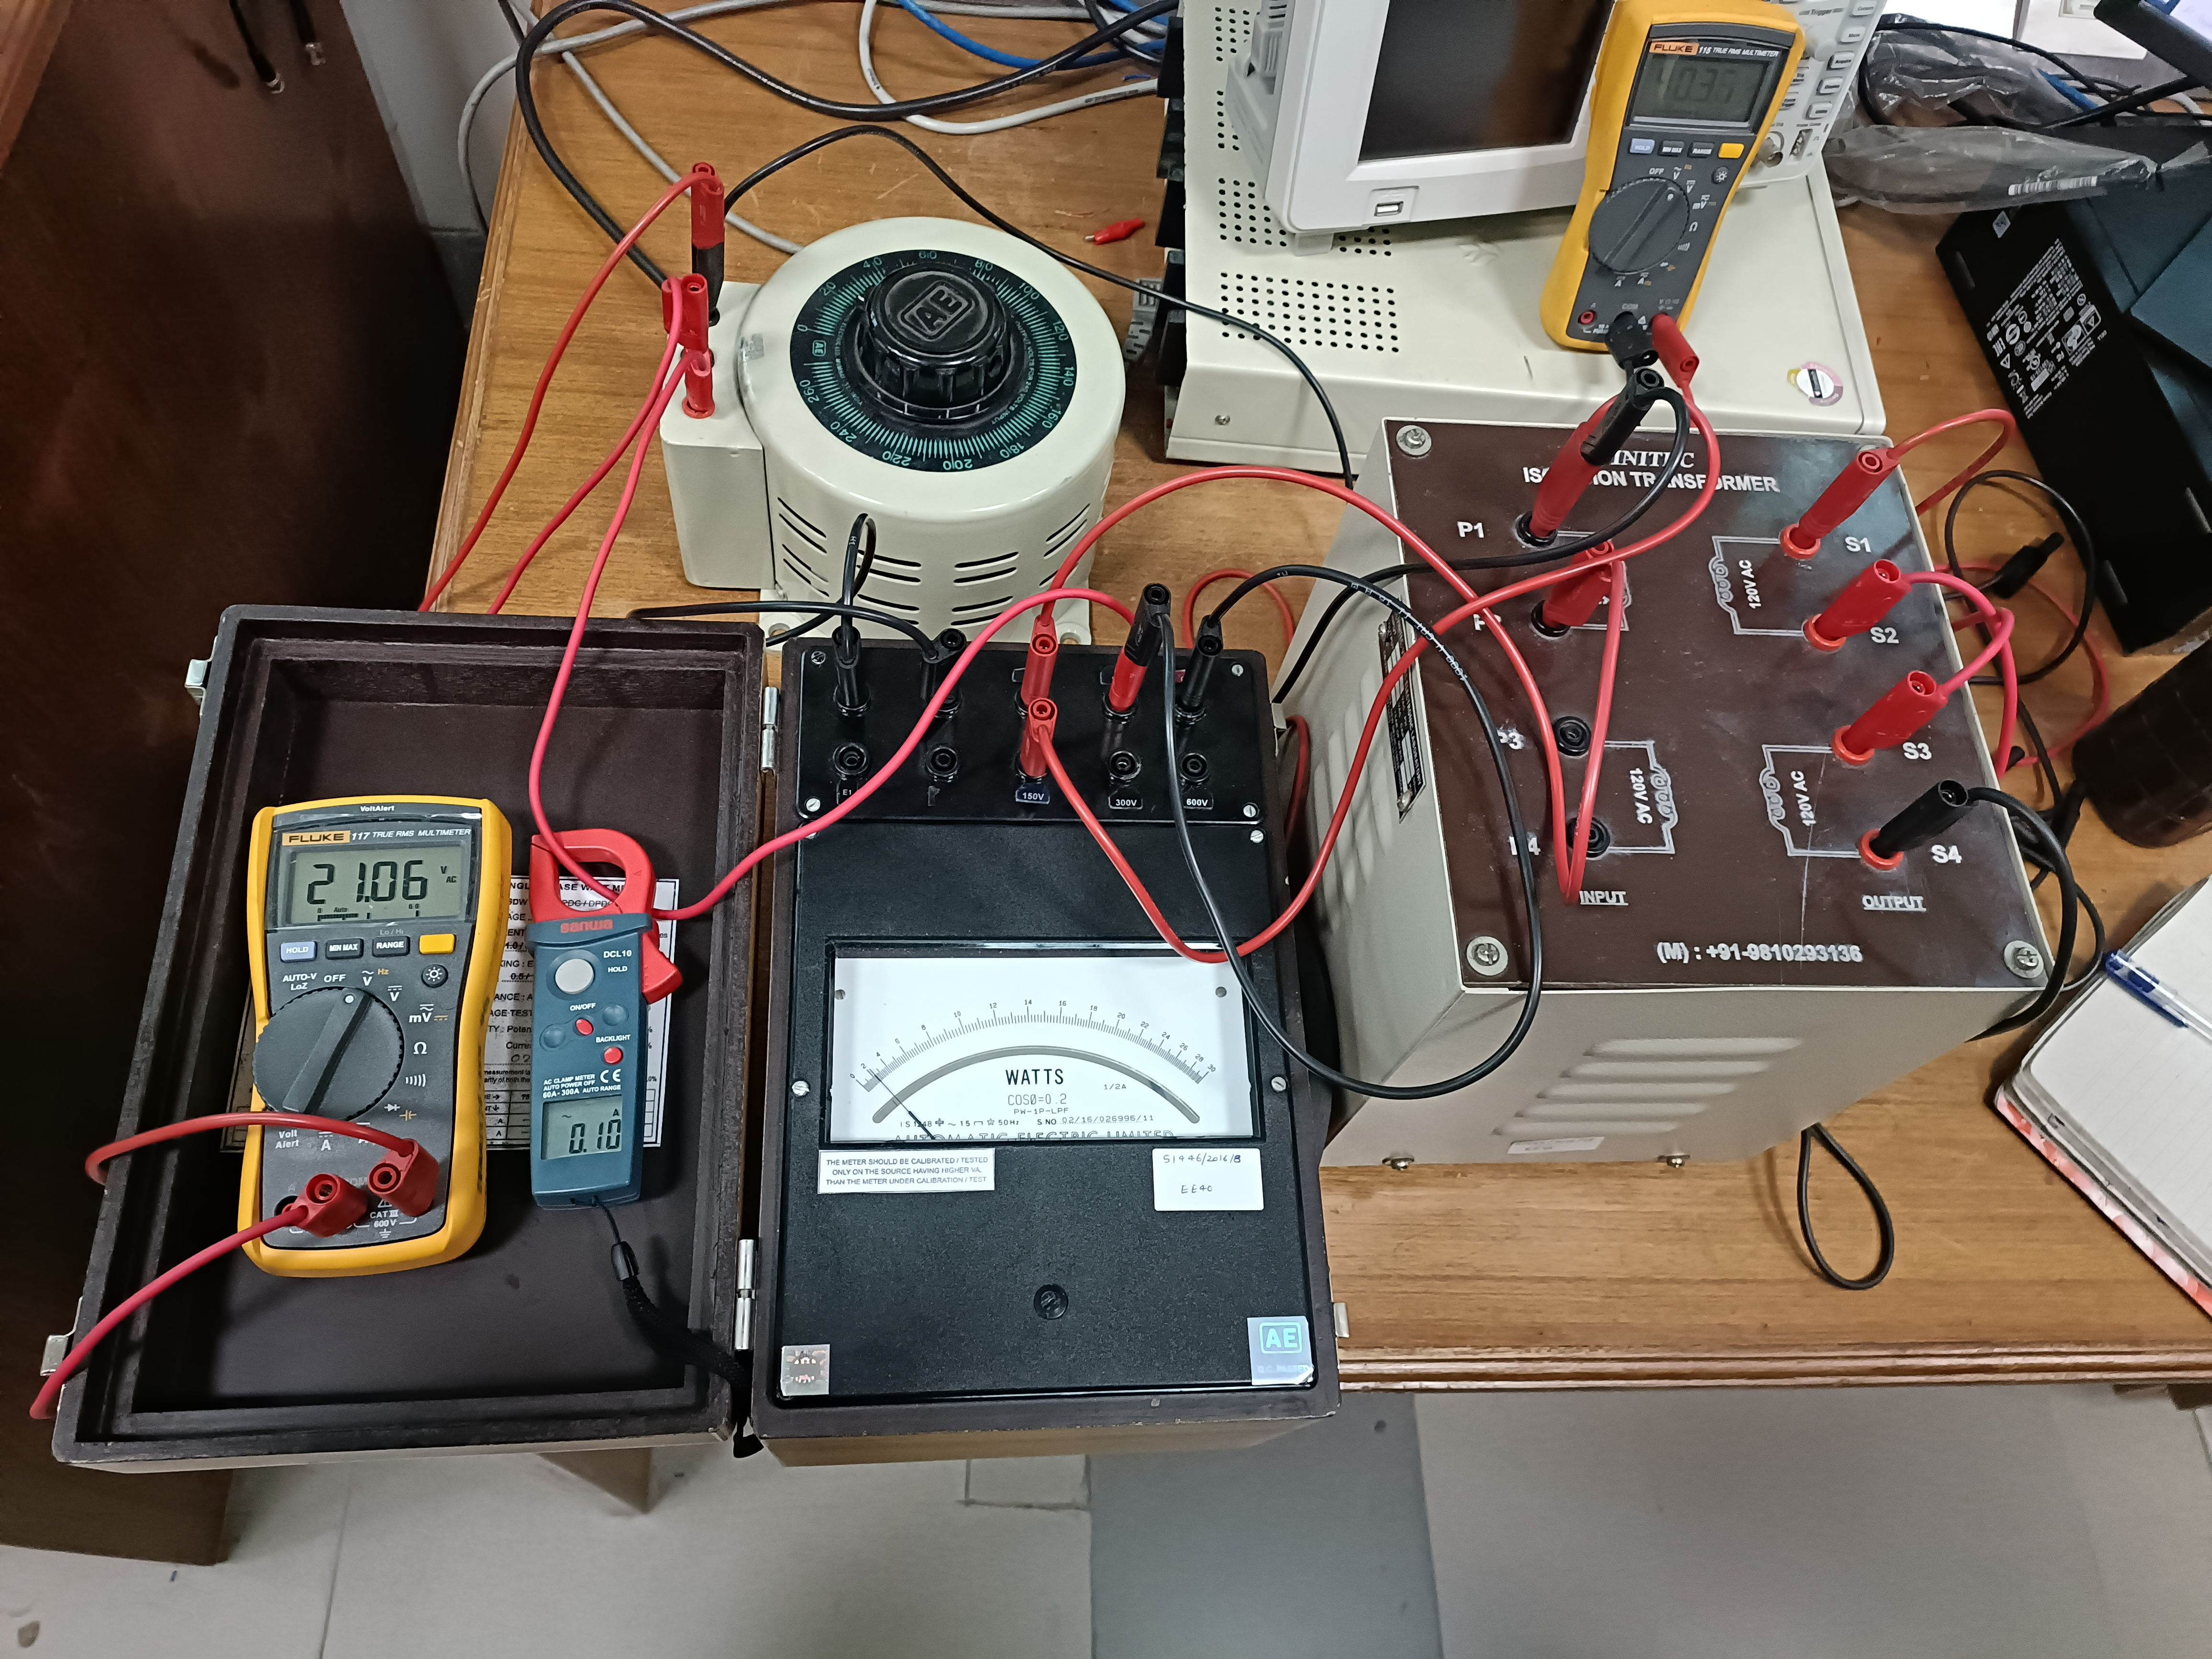
\includegraphics[width=1\columnwidth, height=200px]{IMG20220524154259.jpg}} \\ \vspace{5px}
Open Circuit Test\\

\vspace{20px}

\hline

\vspace{20px}
Short Circuit Test \\
\vspace{5px}
\fcolorbox{black}{white}{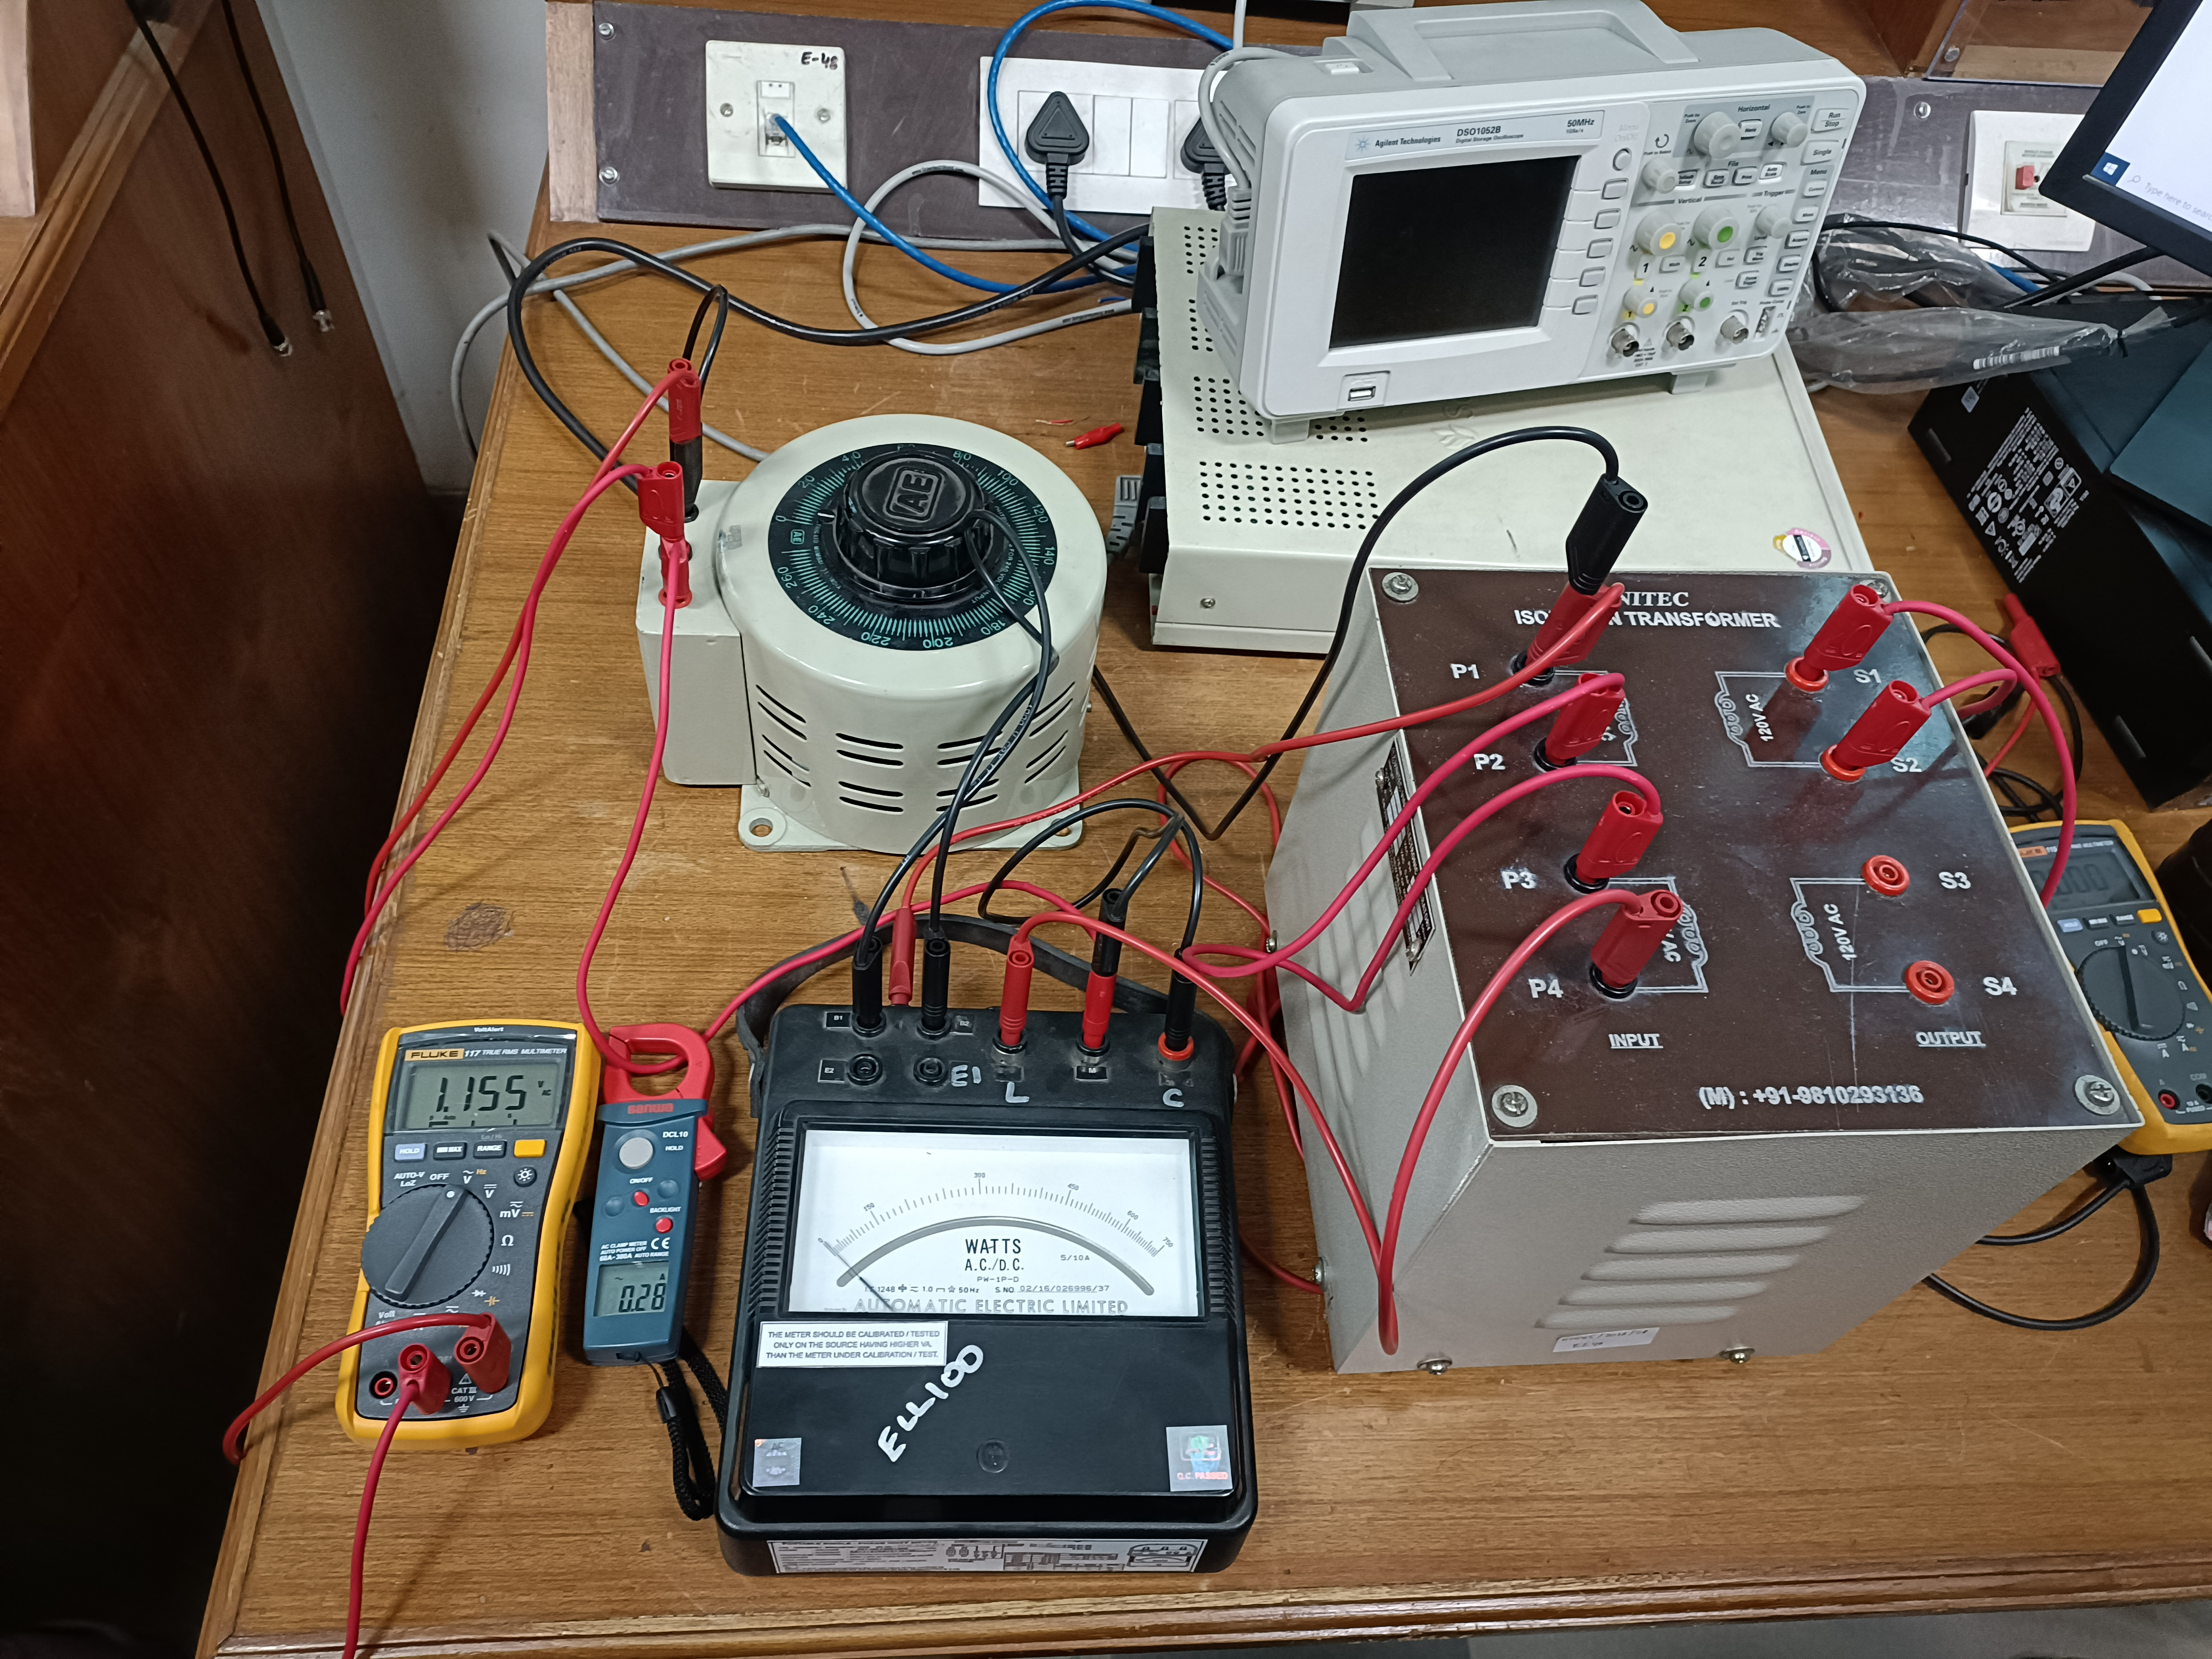
\includegraphics[width=1\columnwidth, height=200px]{IMG20220524155949.jpg}} \\
\end{center}

\newpage


\subsection{Observation}
\vspace{5px}
\begin{center}
OPEN CIRCUIT TEST \\
\vspace{10px}
\begin{tabular}{| V | c | c | c | c |} 
 \hline
    \ & \ & \ & \ & \ \\
    Photo & $V_{Input}$ & $Current$ & $Power$ & $V_{Output}$\\ [1em]
    \hline
    \ & \ & \ & \ & \ \\
    \fcolorbox{black}{yellow!15}{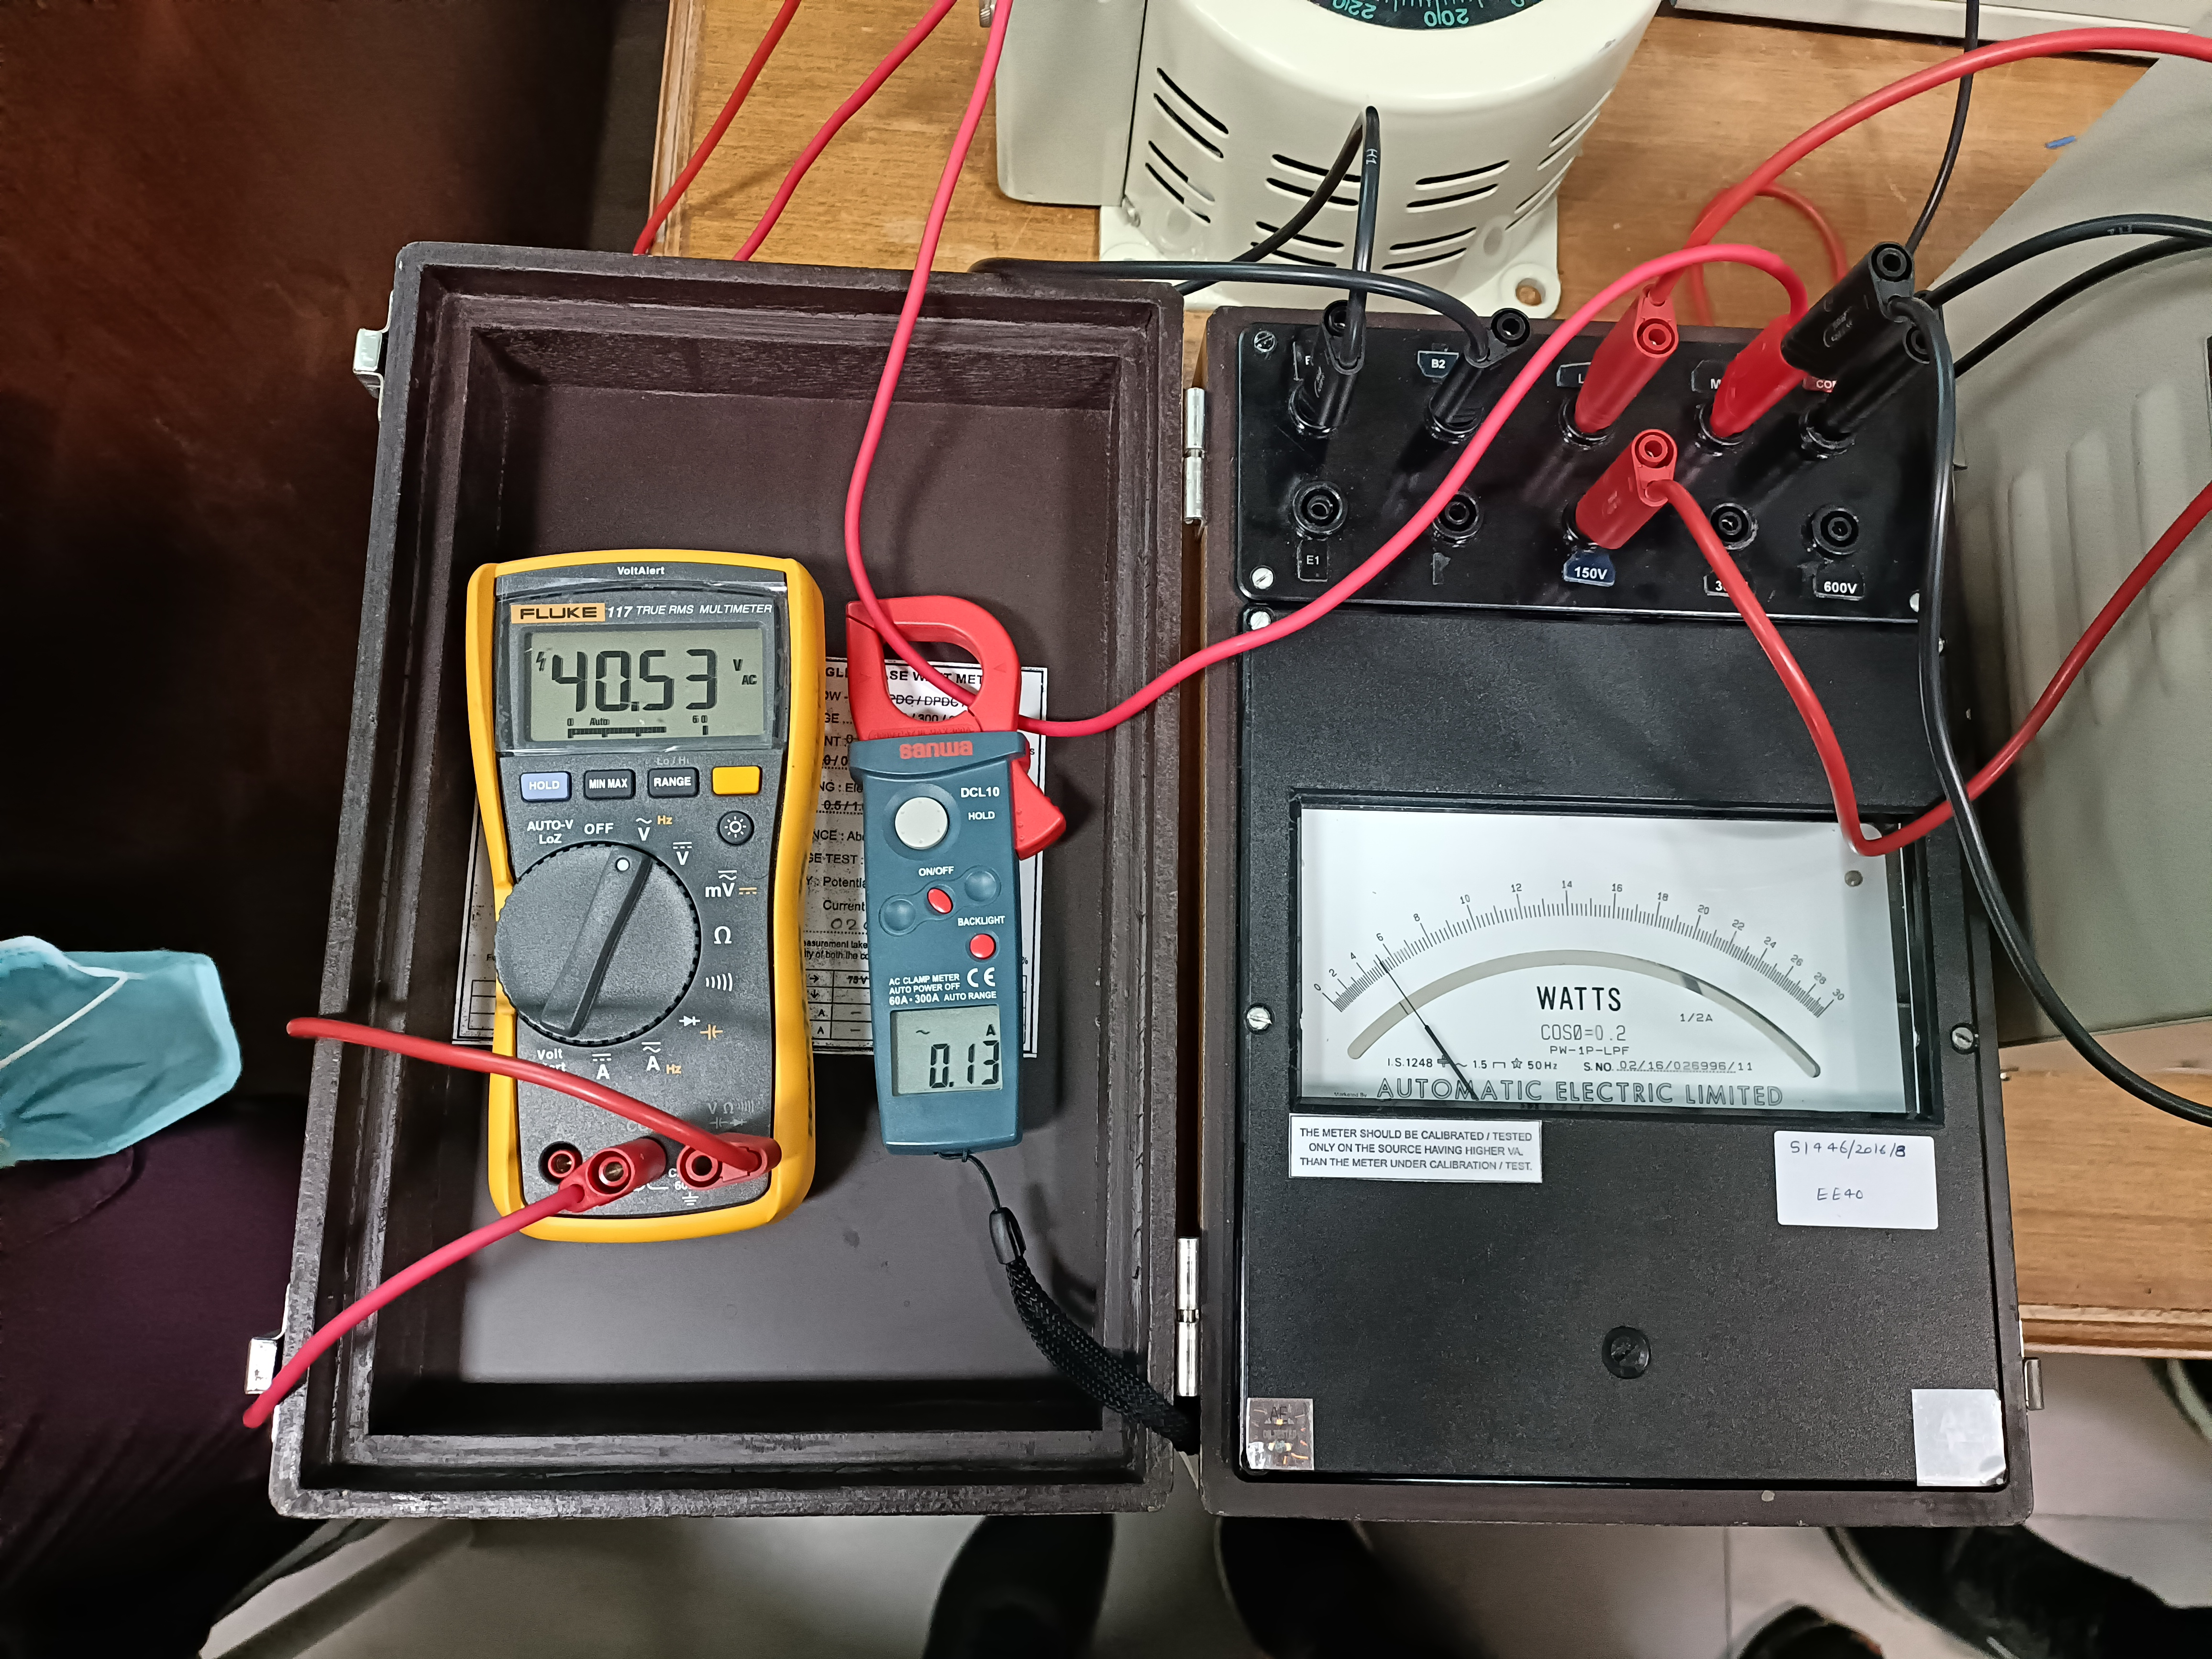
\includegraphics[width=0.35\textwidth]{IMG20220524154544.jpg}} & 40.53V & 0.13A & 5.2W & 78.8V\\
    \vspace{10px}
    \fcolorbox{black}{yellow!15}{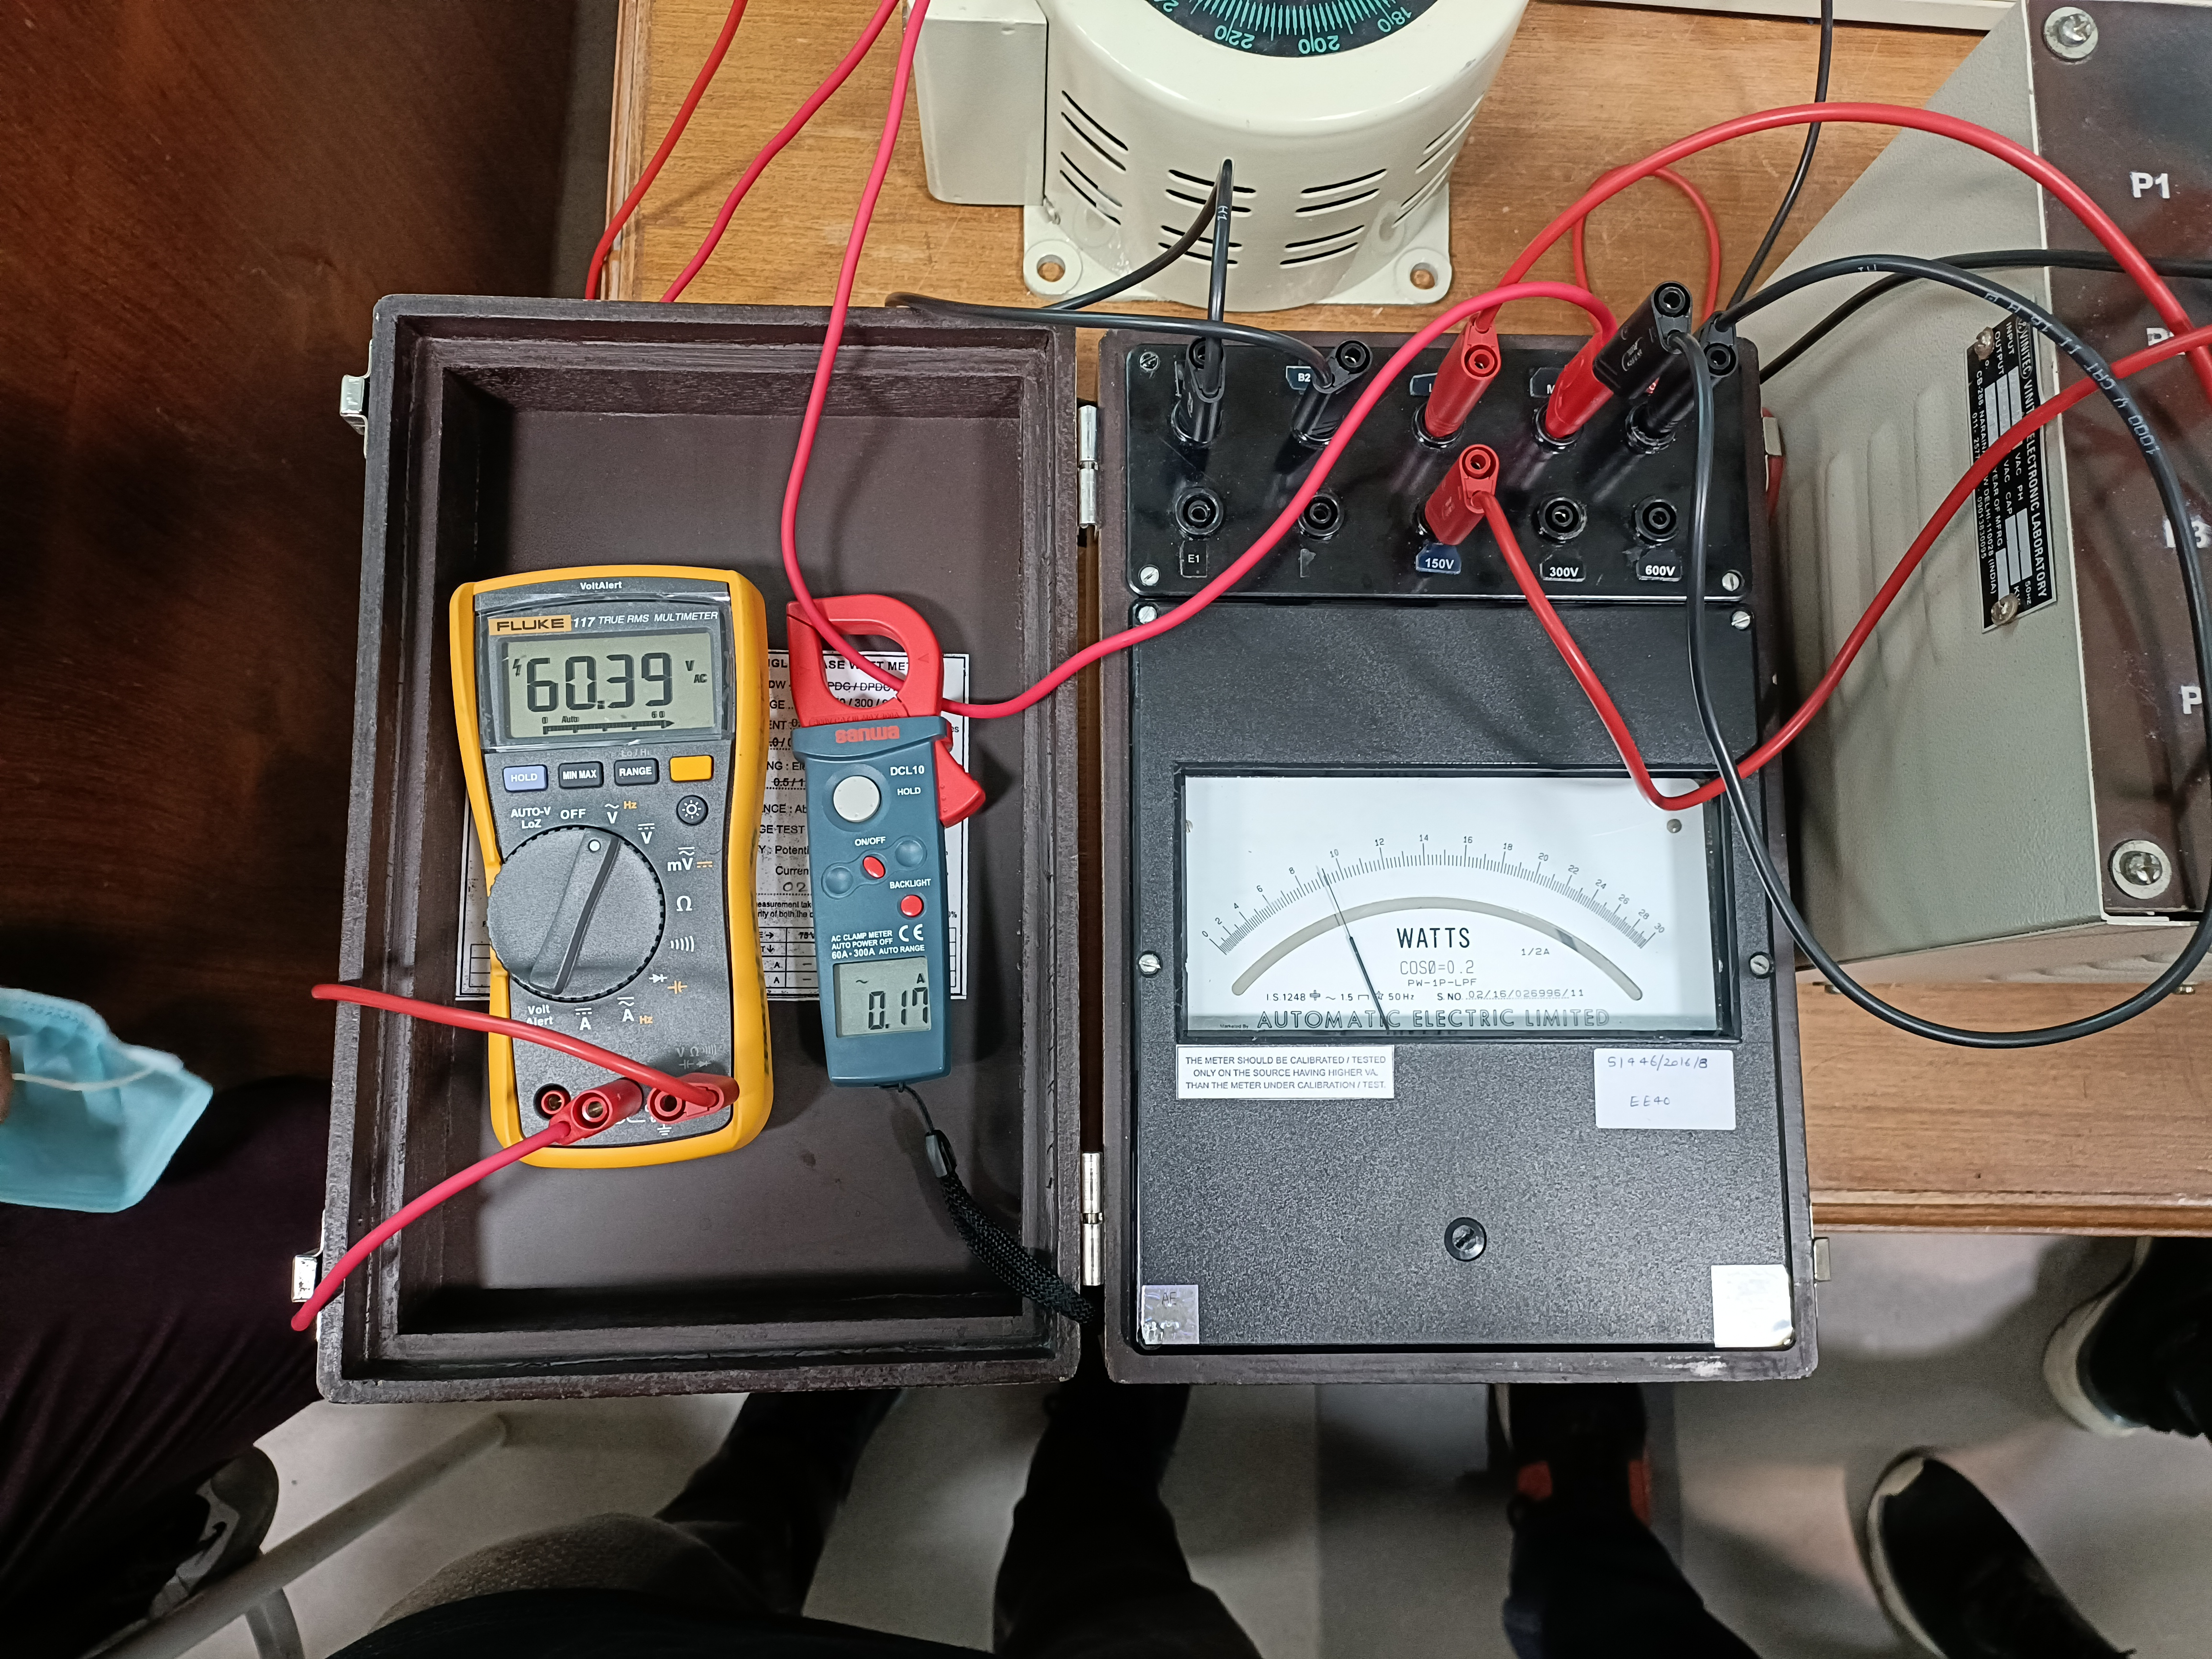
\includegraphics[width=0.35\textwidth]{IMG20220524154613.jpg}} & 60.4V & 0.17A & 9.2W & 118.5V\\
    \vspace{10px}
    \fcolorbox{black}{yellow!15}{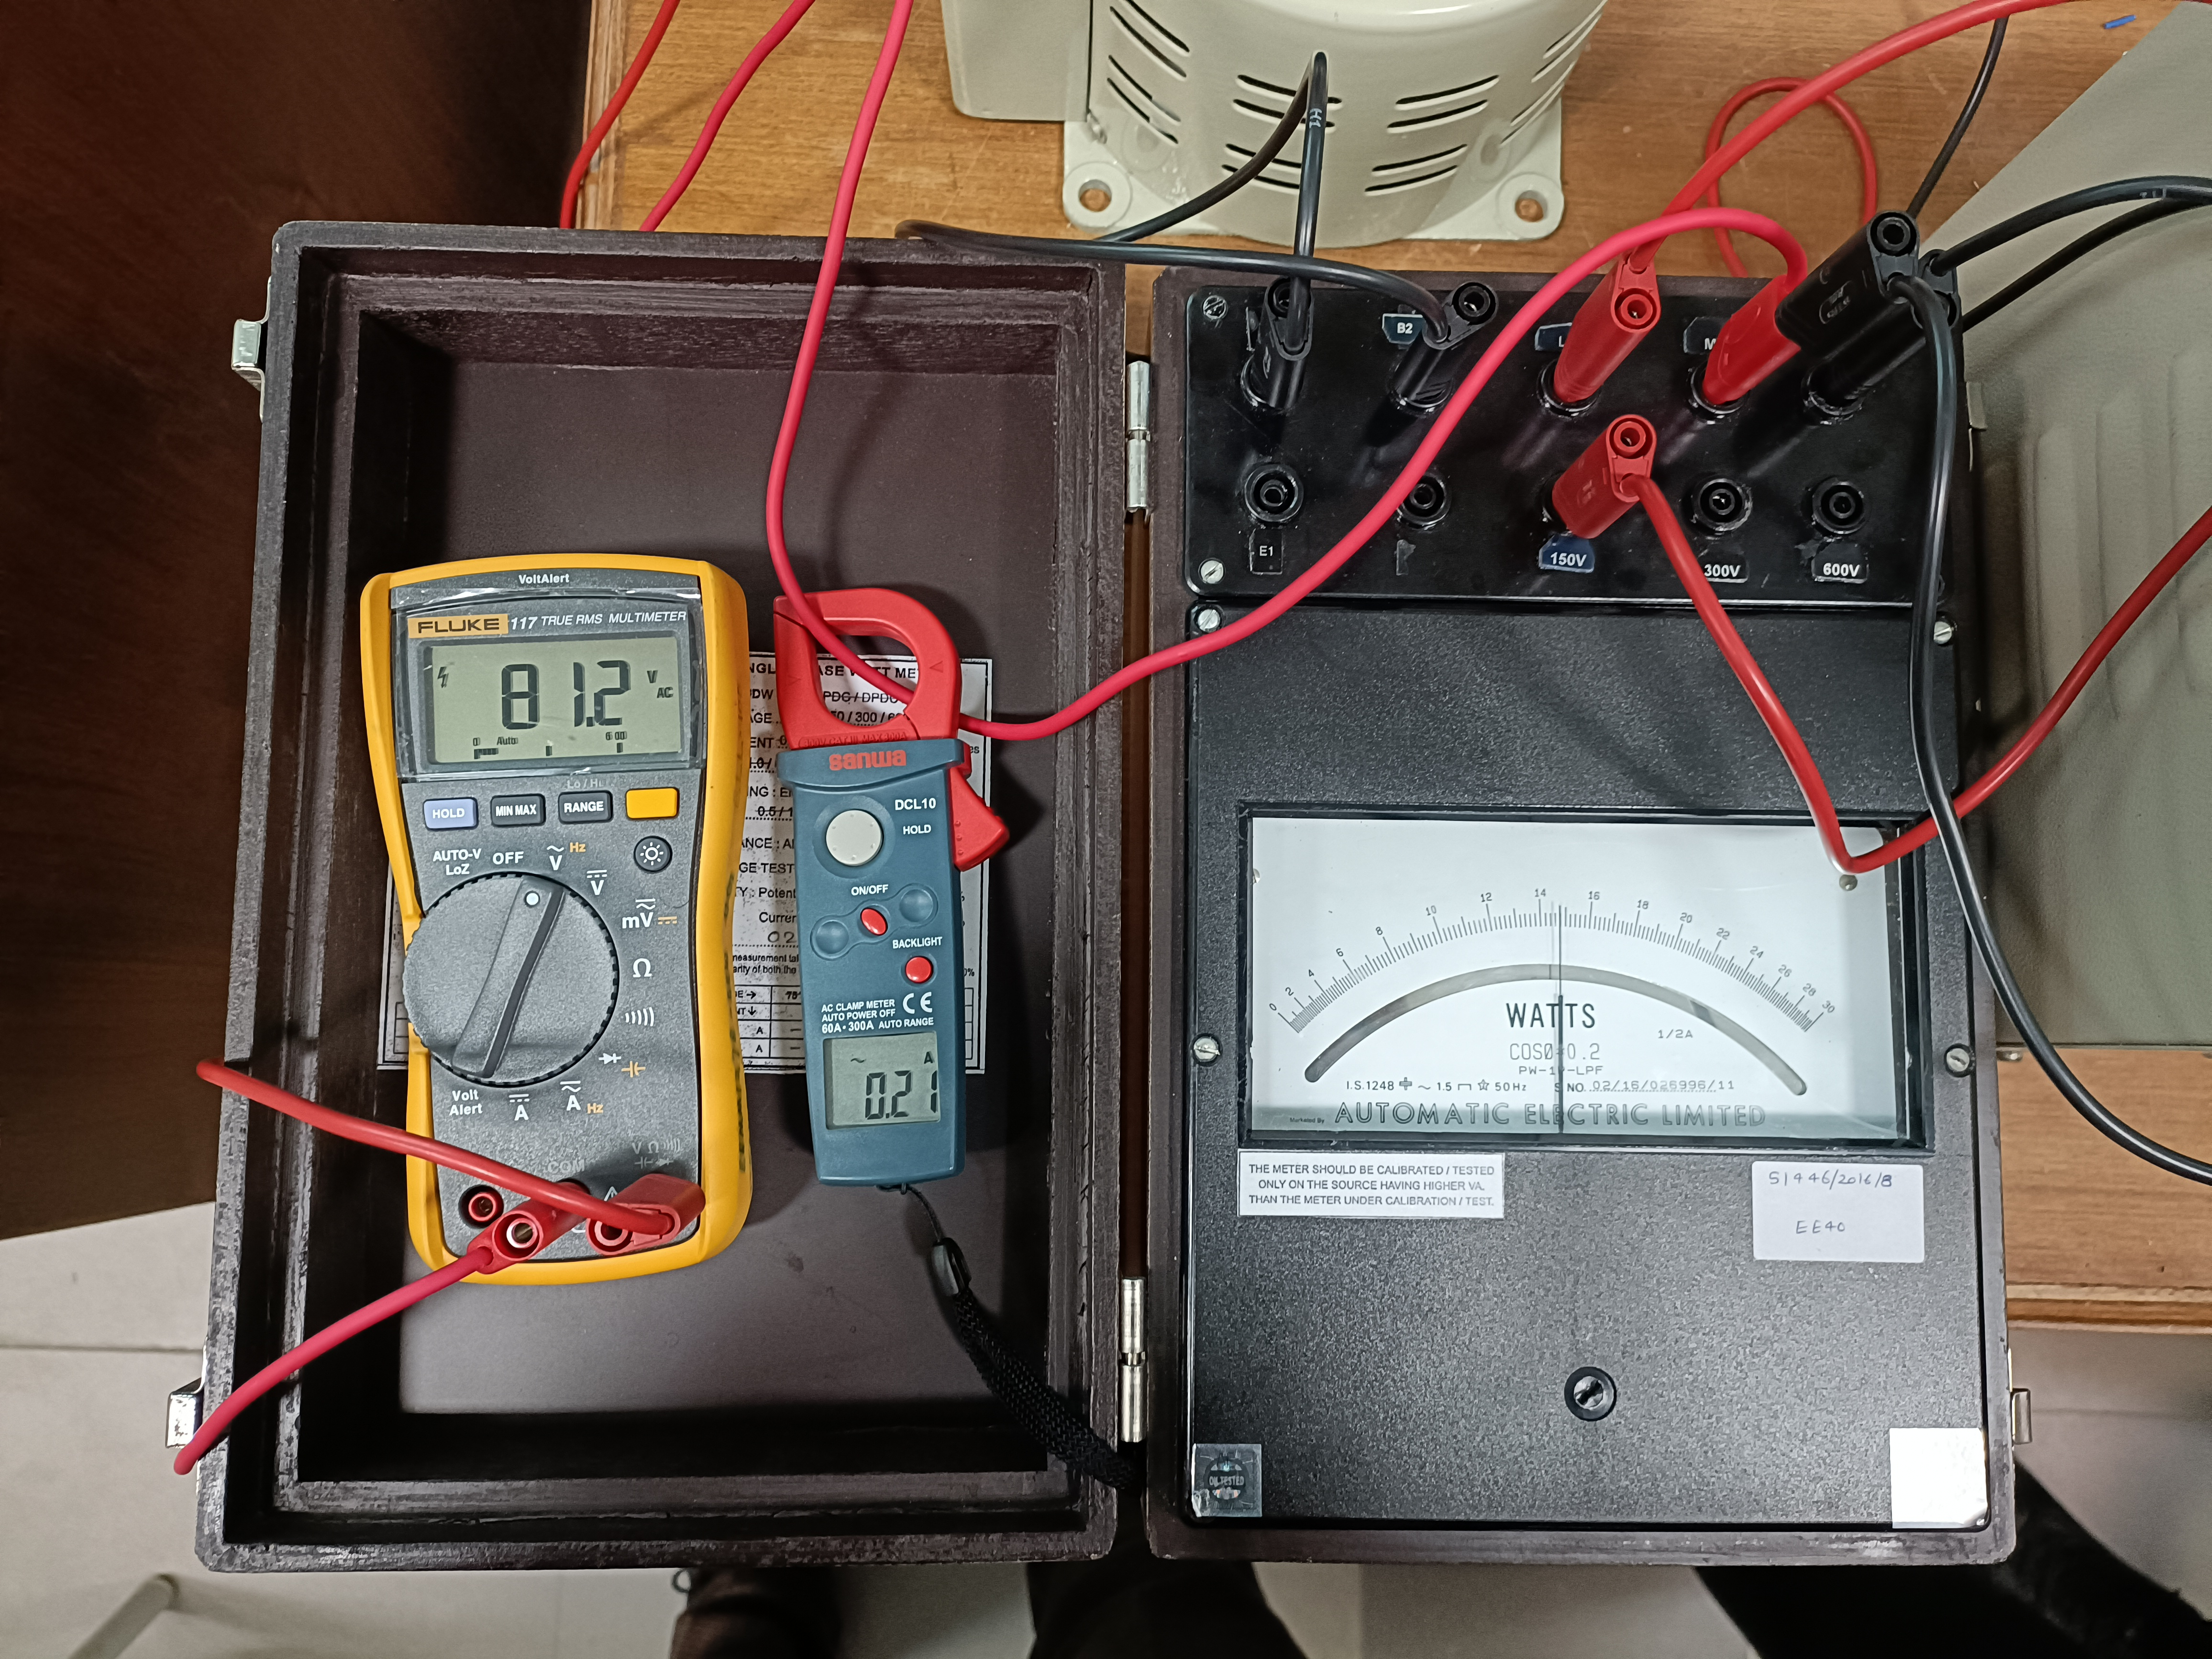
\includegraphics[width=0.35\textwidth]{IMG20220524154648.jpg}} & 81.3V & 0.21A & 14.6W & 159.7V\\
    \vspace{10px}
    \fcolorbox{black}{yellow!15}{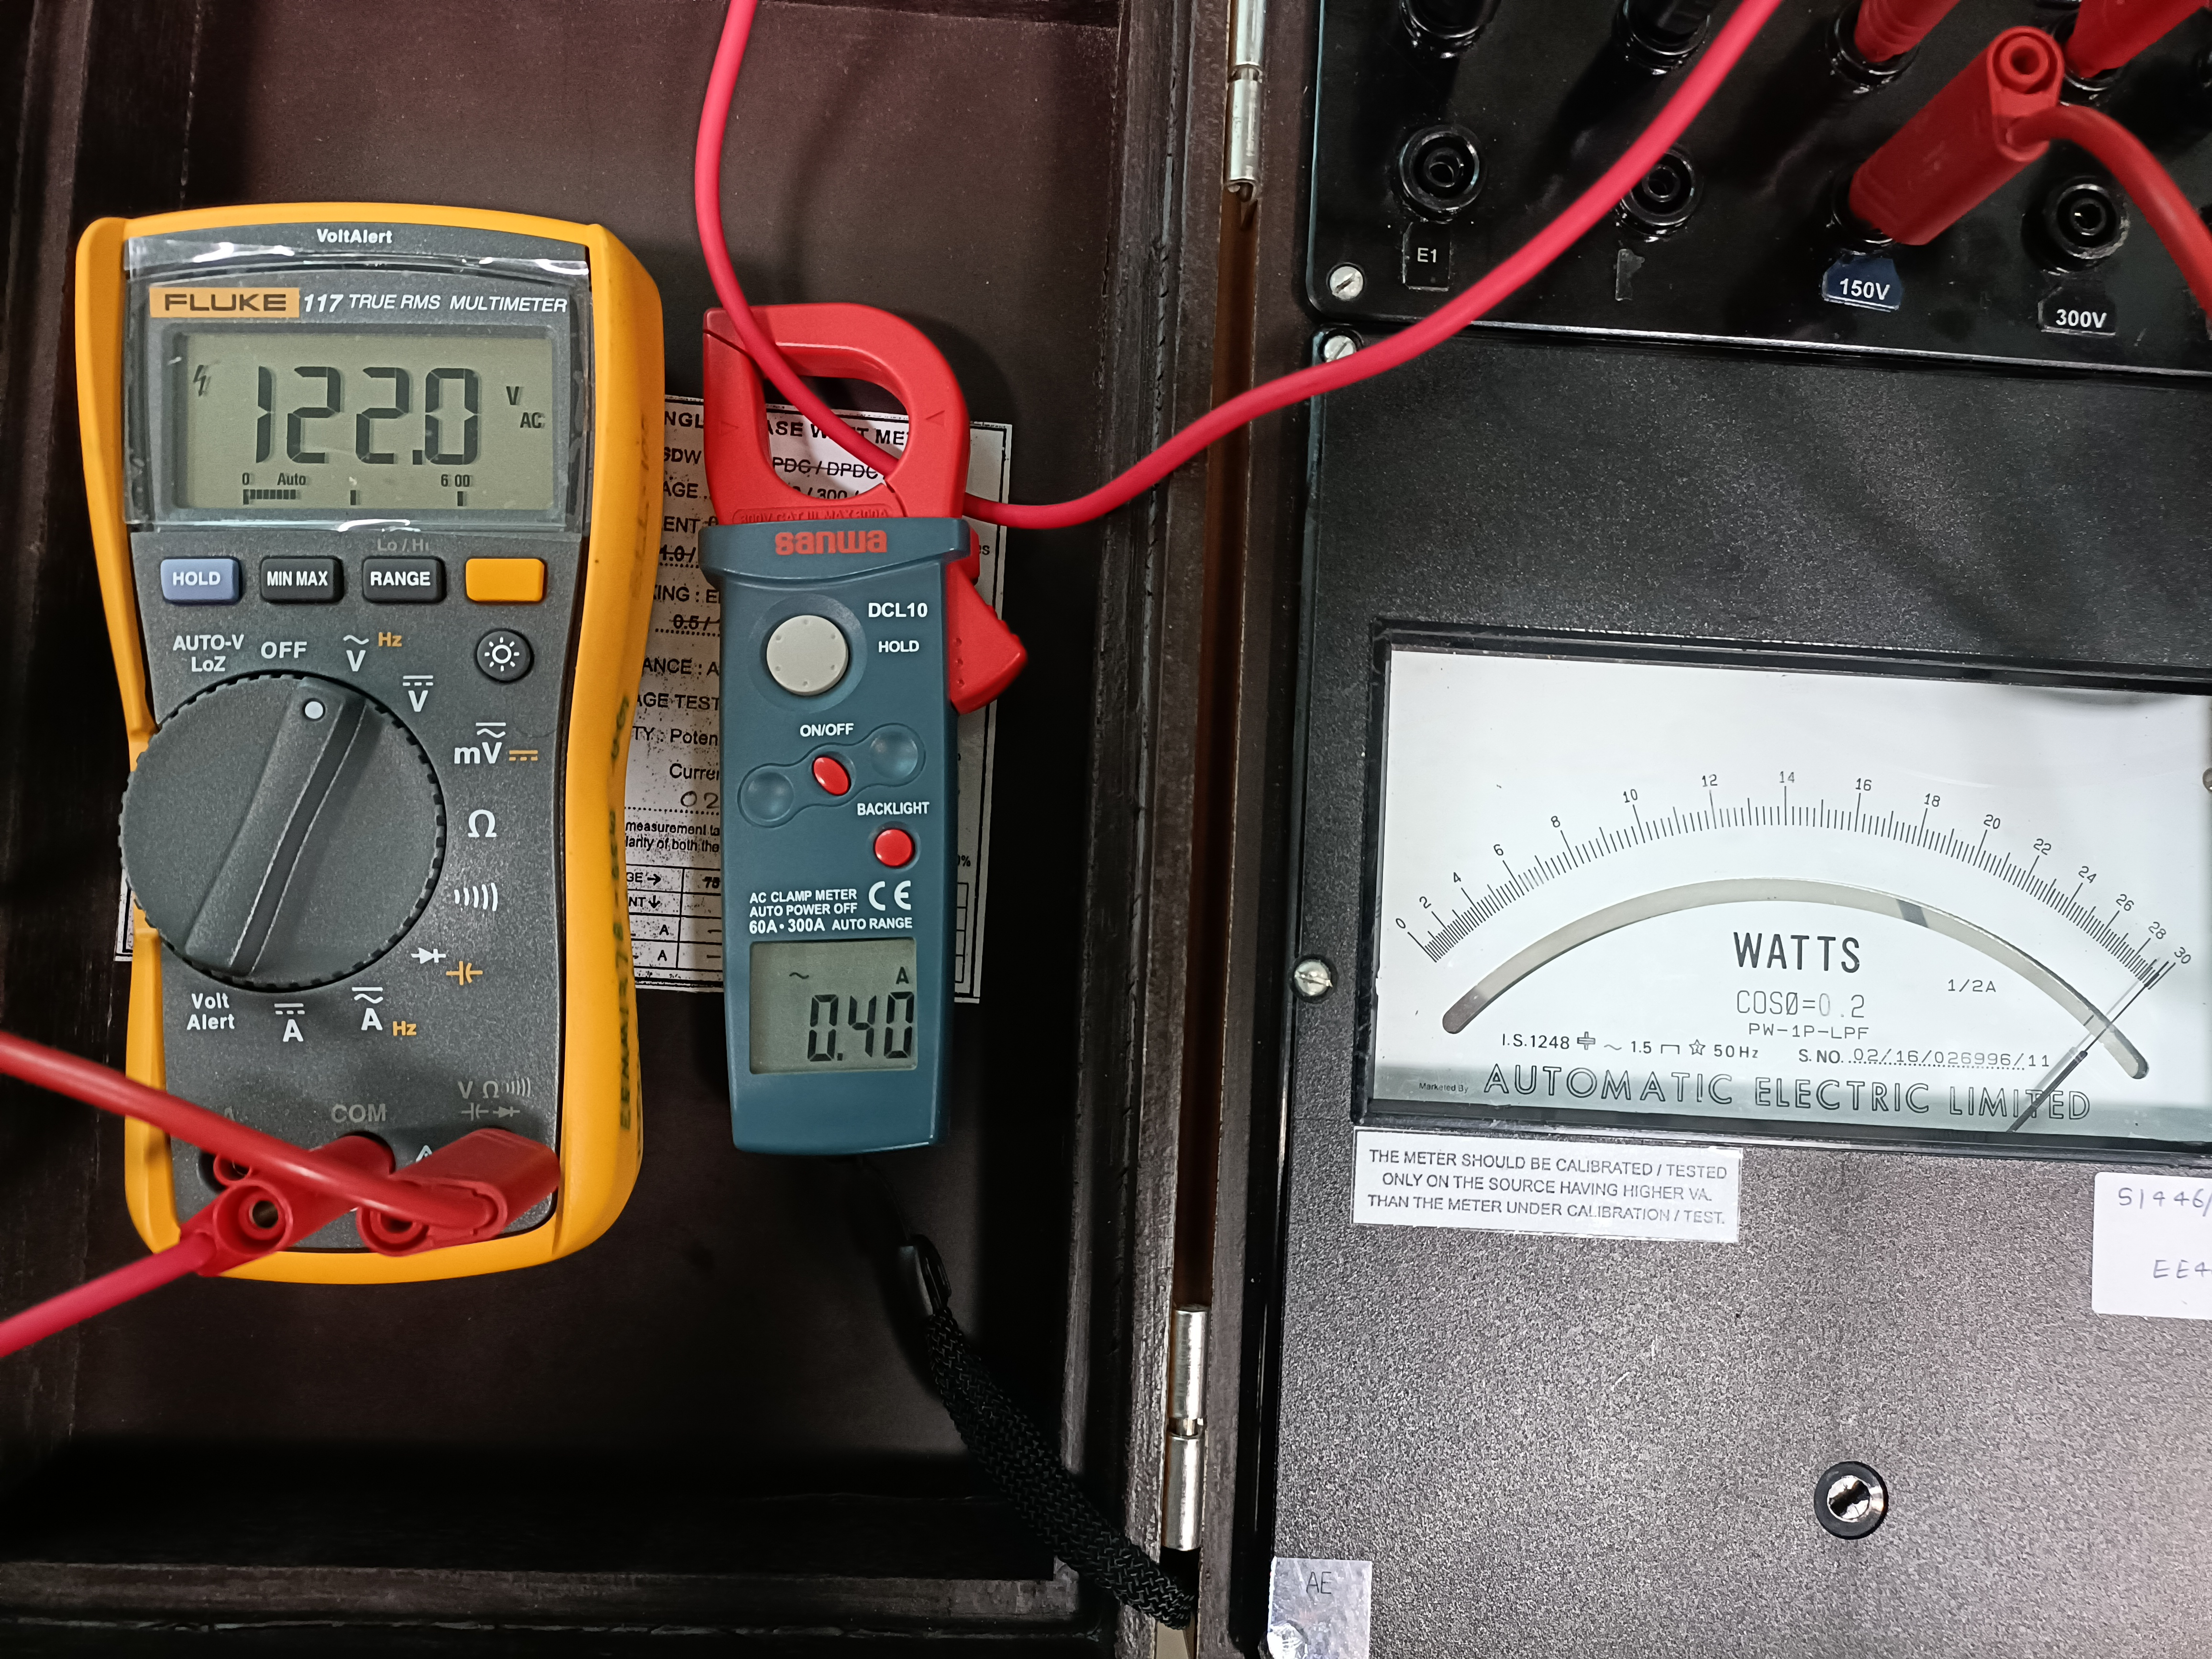
\includegraphics[width=0.35\textwidth]{IMG20220524154803.jpg}} & 122.0V & 0.4A & 29.5W & 239.5V\\
    \ & \ & \ & \ & \ \\
 \hline
\end{tabular}
\end{center}
\newpage
\vspace{5px}
\begin{center}
SHORT CIRCUIT TEST \\
\vspace{10px}
\begin{tabular}{| V | c | c | c |} 
 \hline
    \ & \ & \ & \ \\
    Photo & $V_{Input}$ & $Current$ & $Power$ \\ [1em]
    \hline
    \ & \ & \ & \ \\
    \fcolorbox{black}{yellow!15}{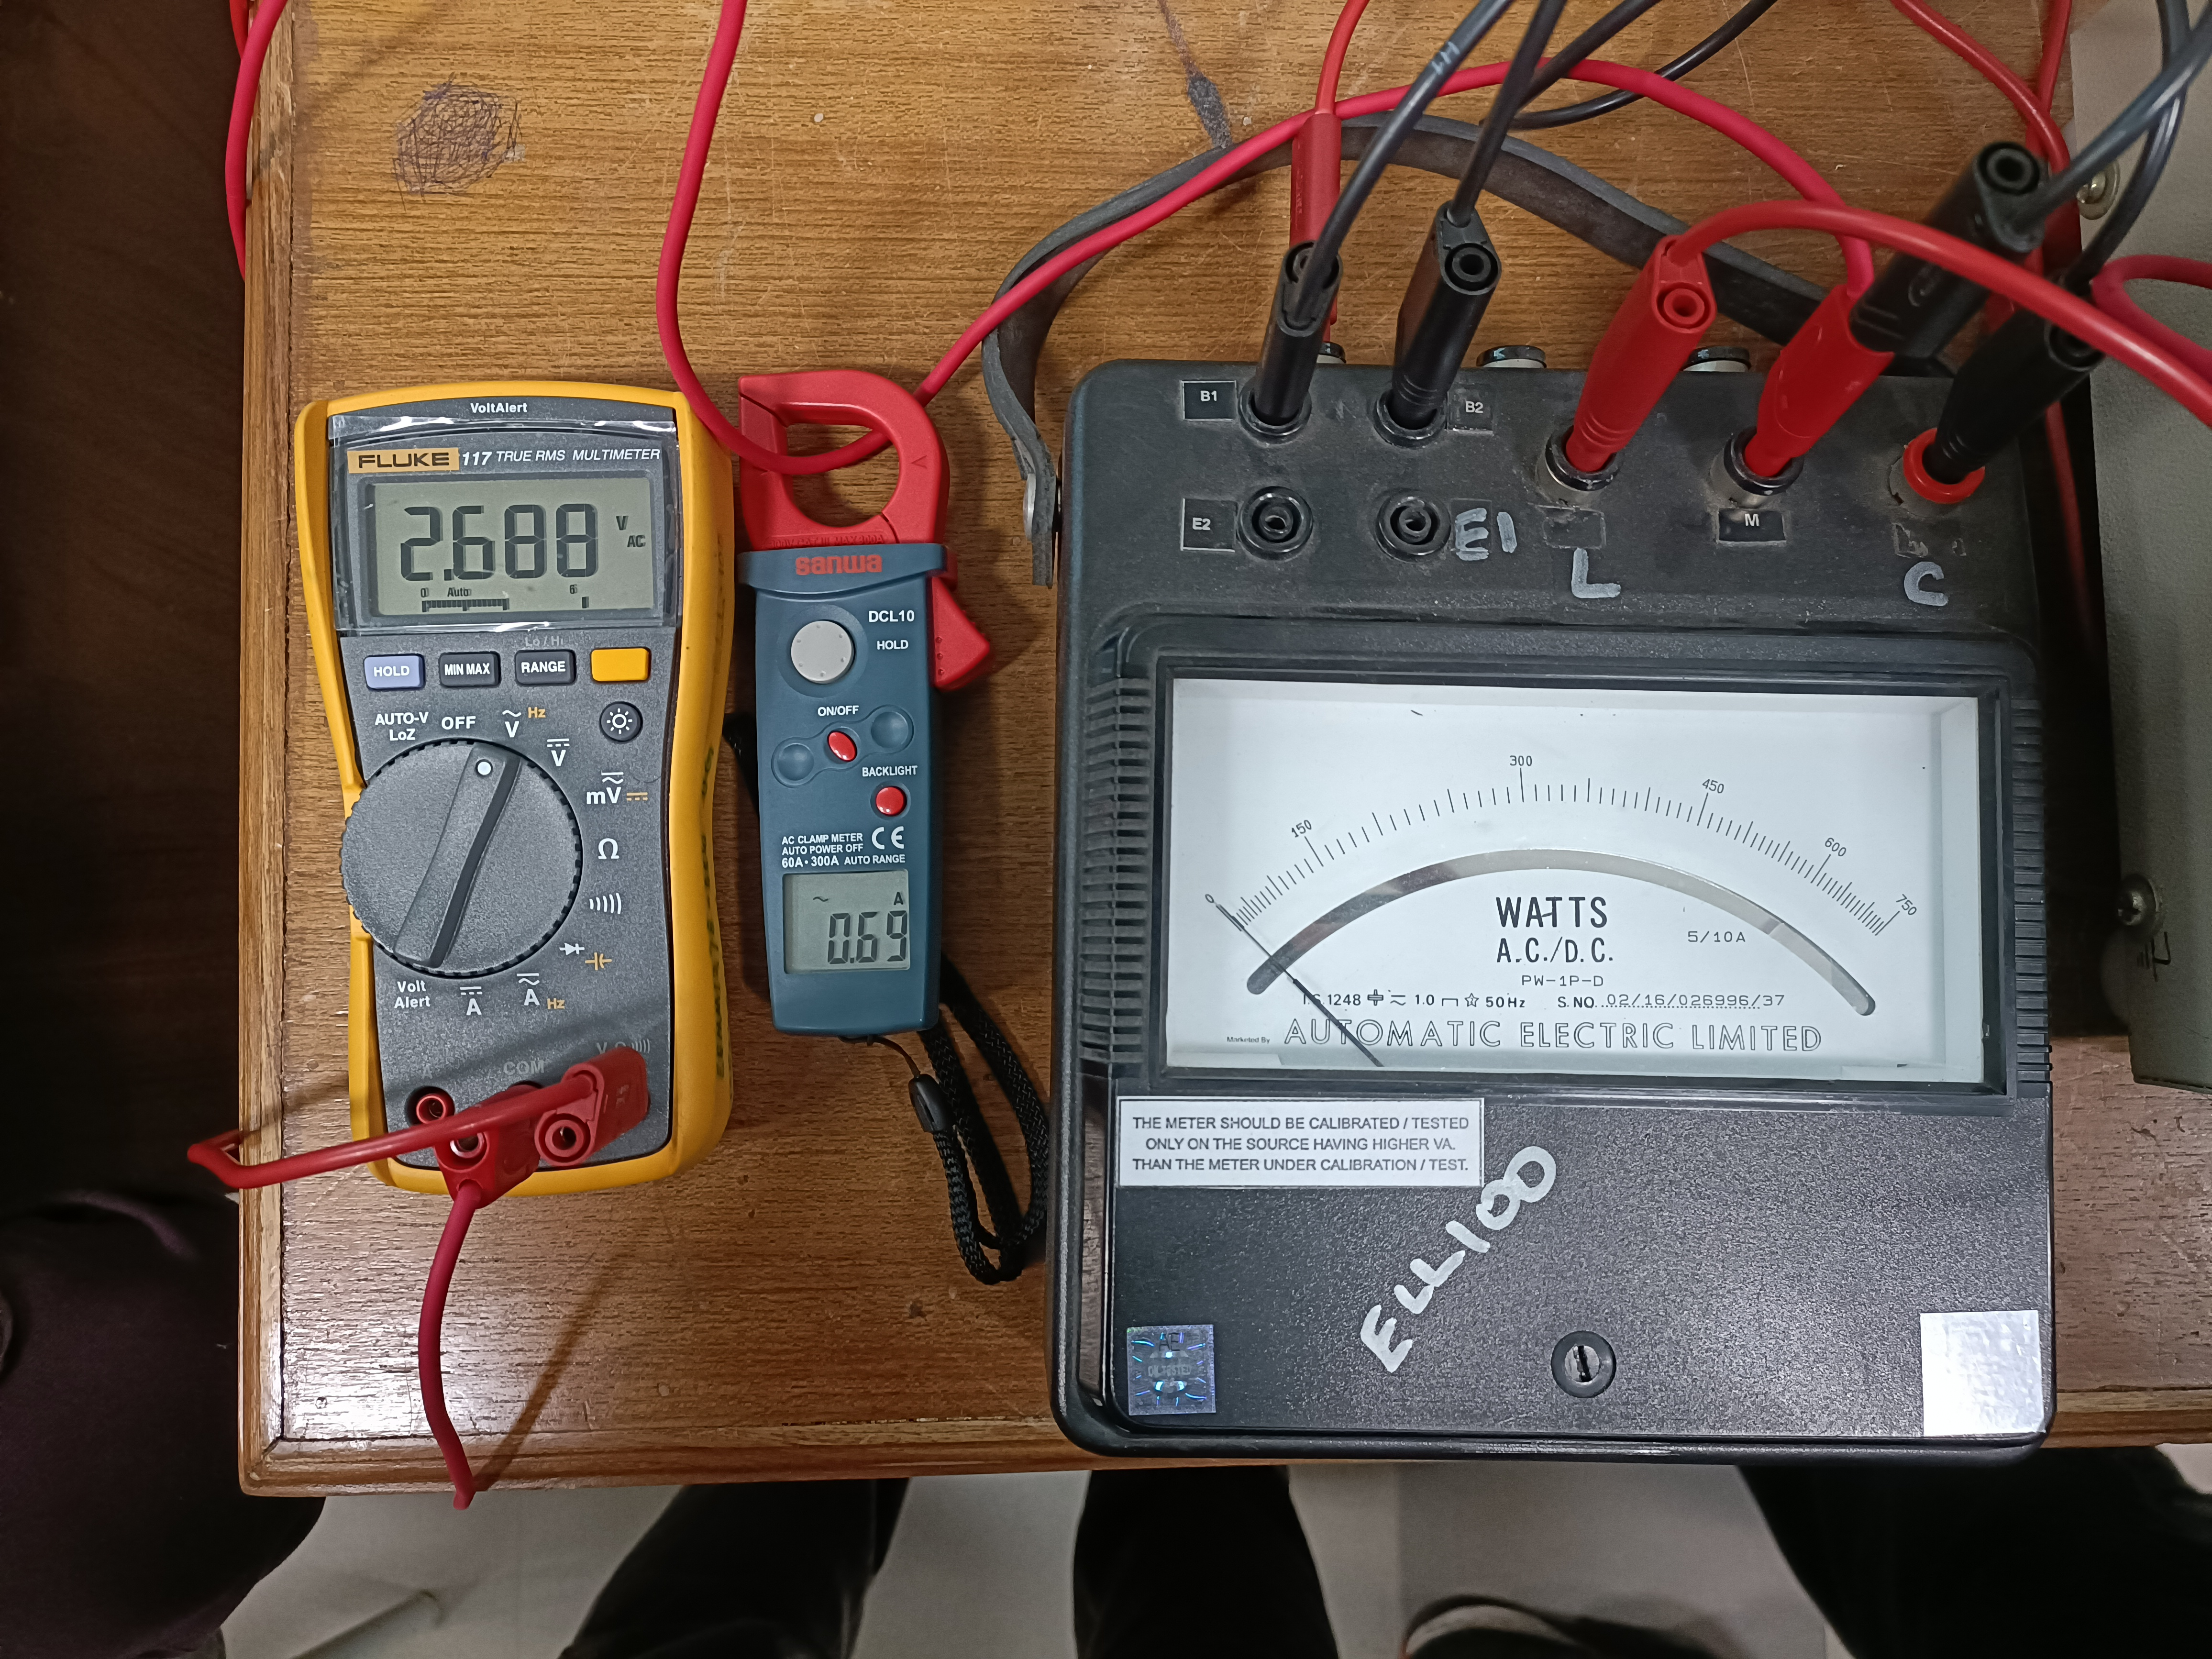
\includegraphics[width=0.35\textwidth]{IMG20220524160019.jpg}} & 2.68V & 0.69A & 0W \\
    \vspace{10px}
    \fcolorbox{black}{yellow!15}{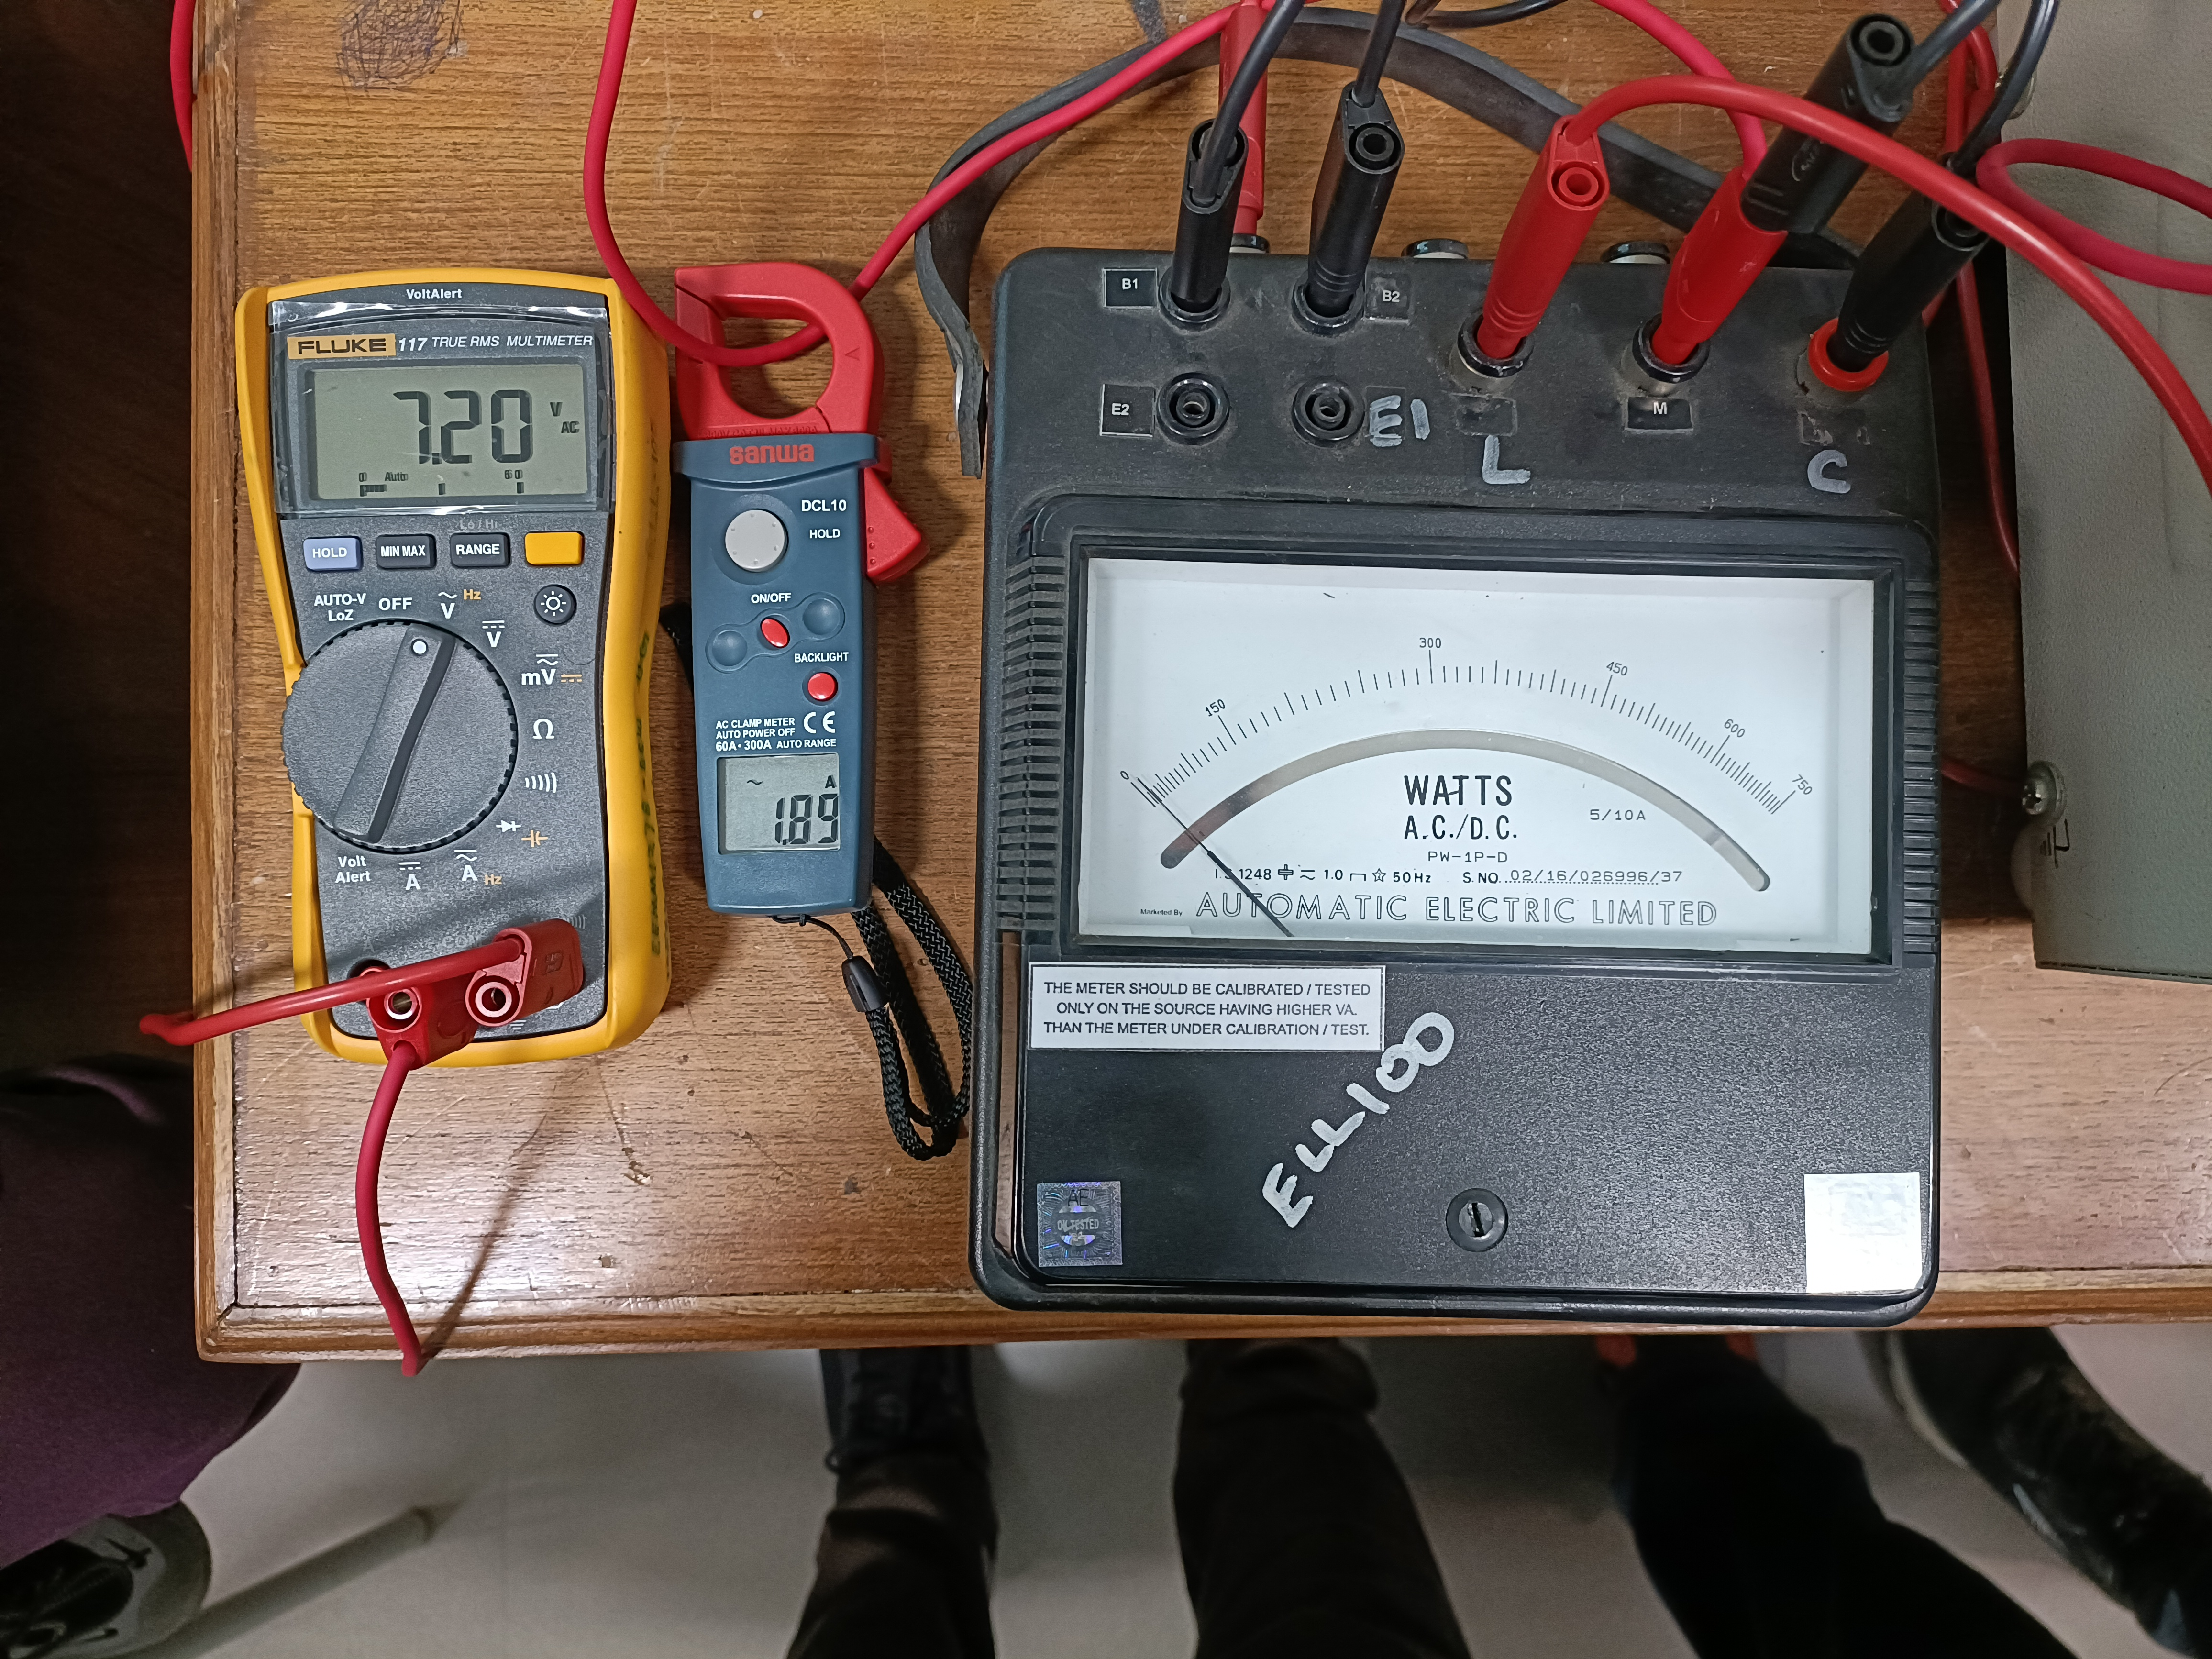
\includegraphics[width=0.35\textwidth]{IMG20220524160046.jpg}} & 7.15V & 1.88A & 10W \\
    \vspace{10px}
    \fcolorbox{black}{yellow!15}{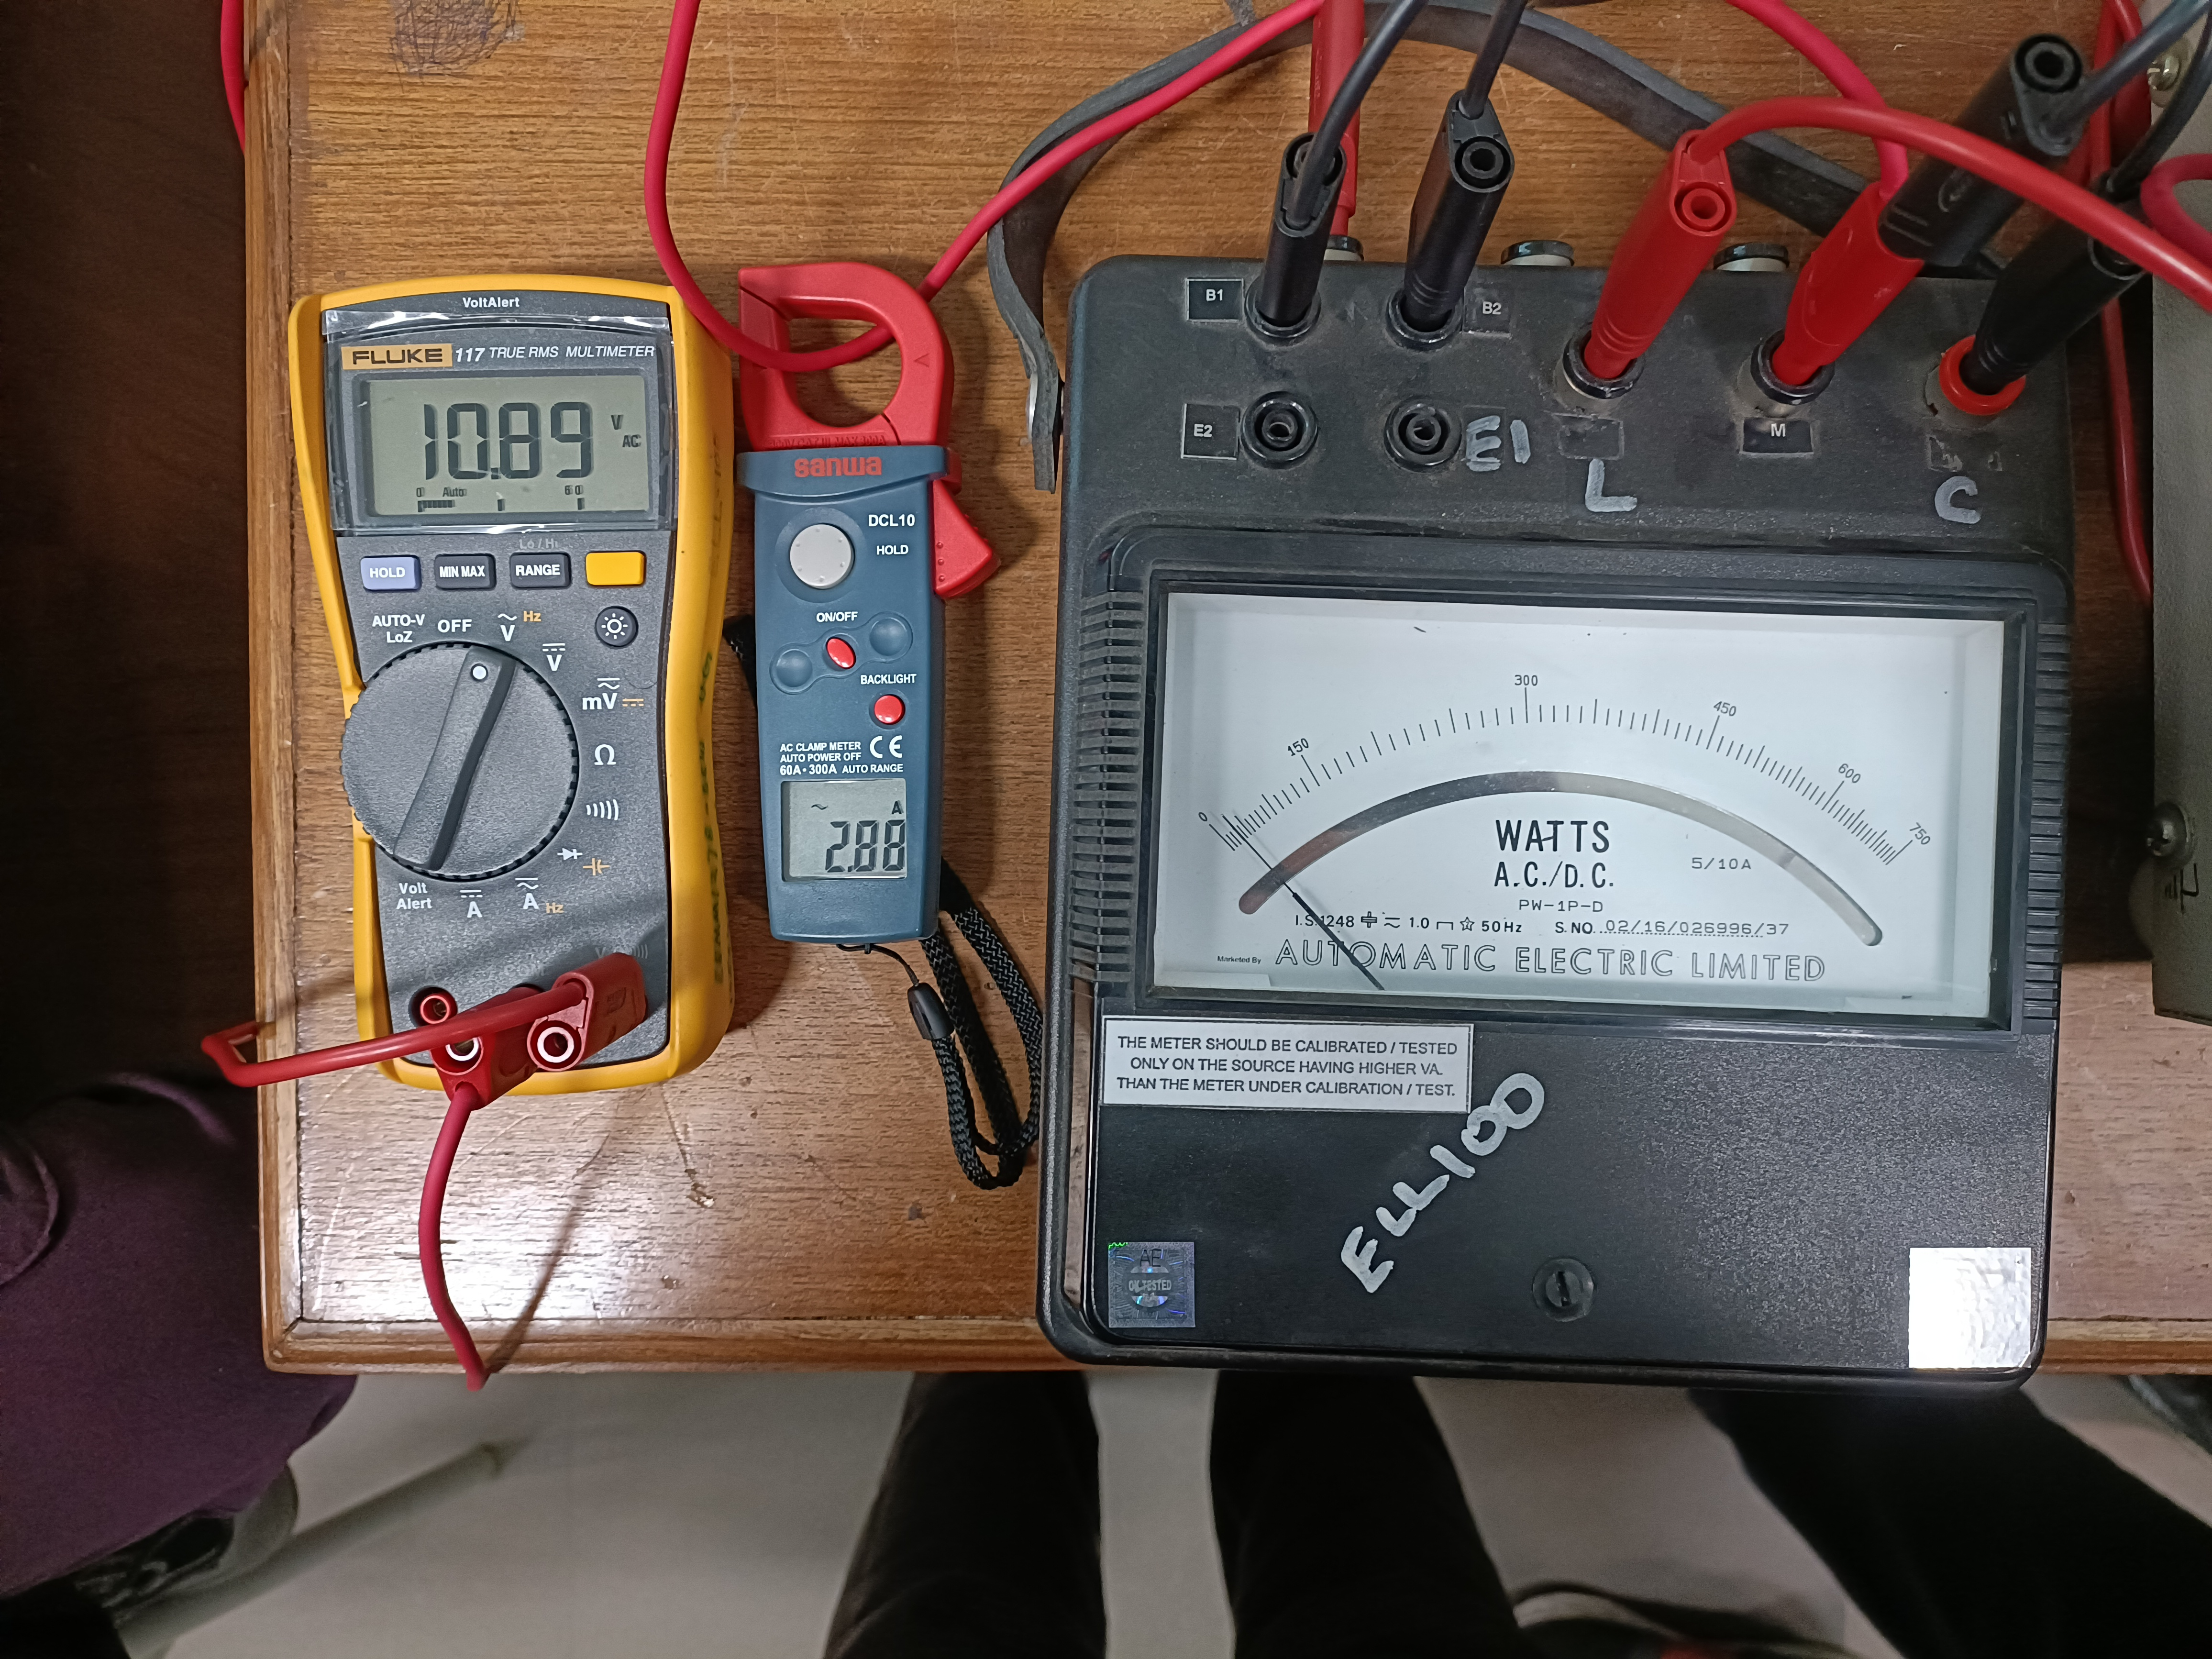
\includegraphics[width=0.35\textwidth]{IMG20220524160111.jpg}} & 10.9V & 2.89A & 30W \\
    \vspace{10px}
    \fcolorbox{black}{yellow!15}{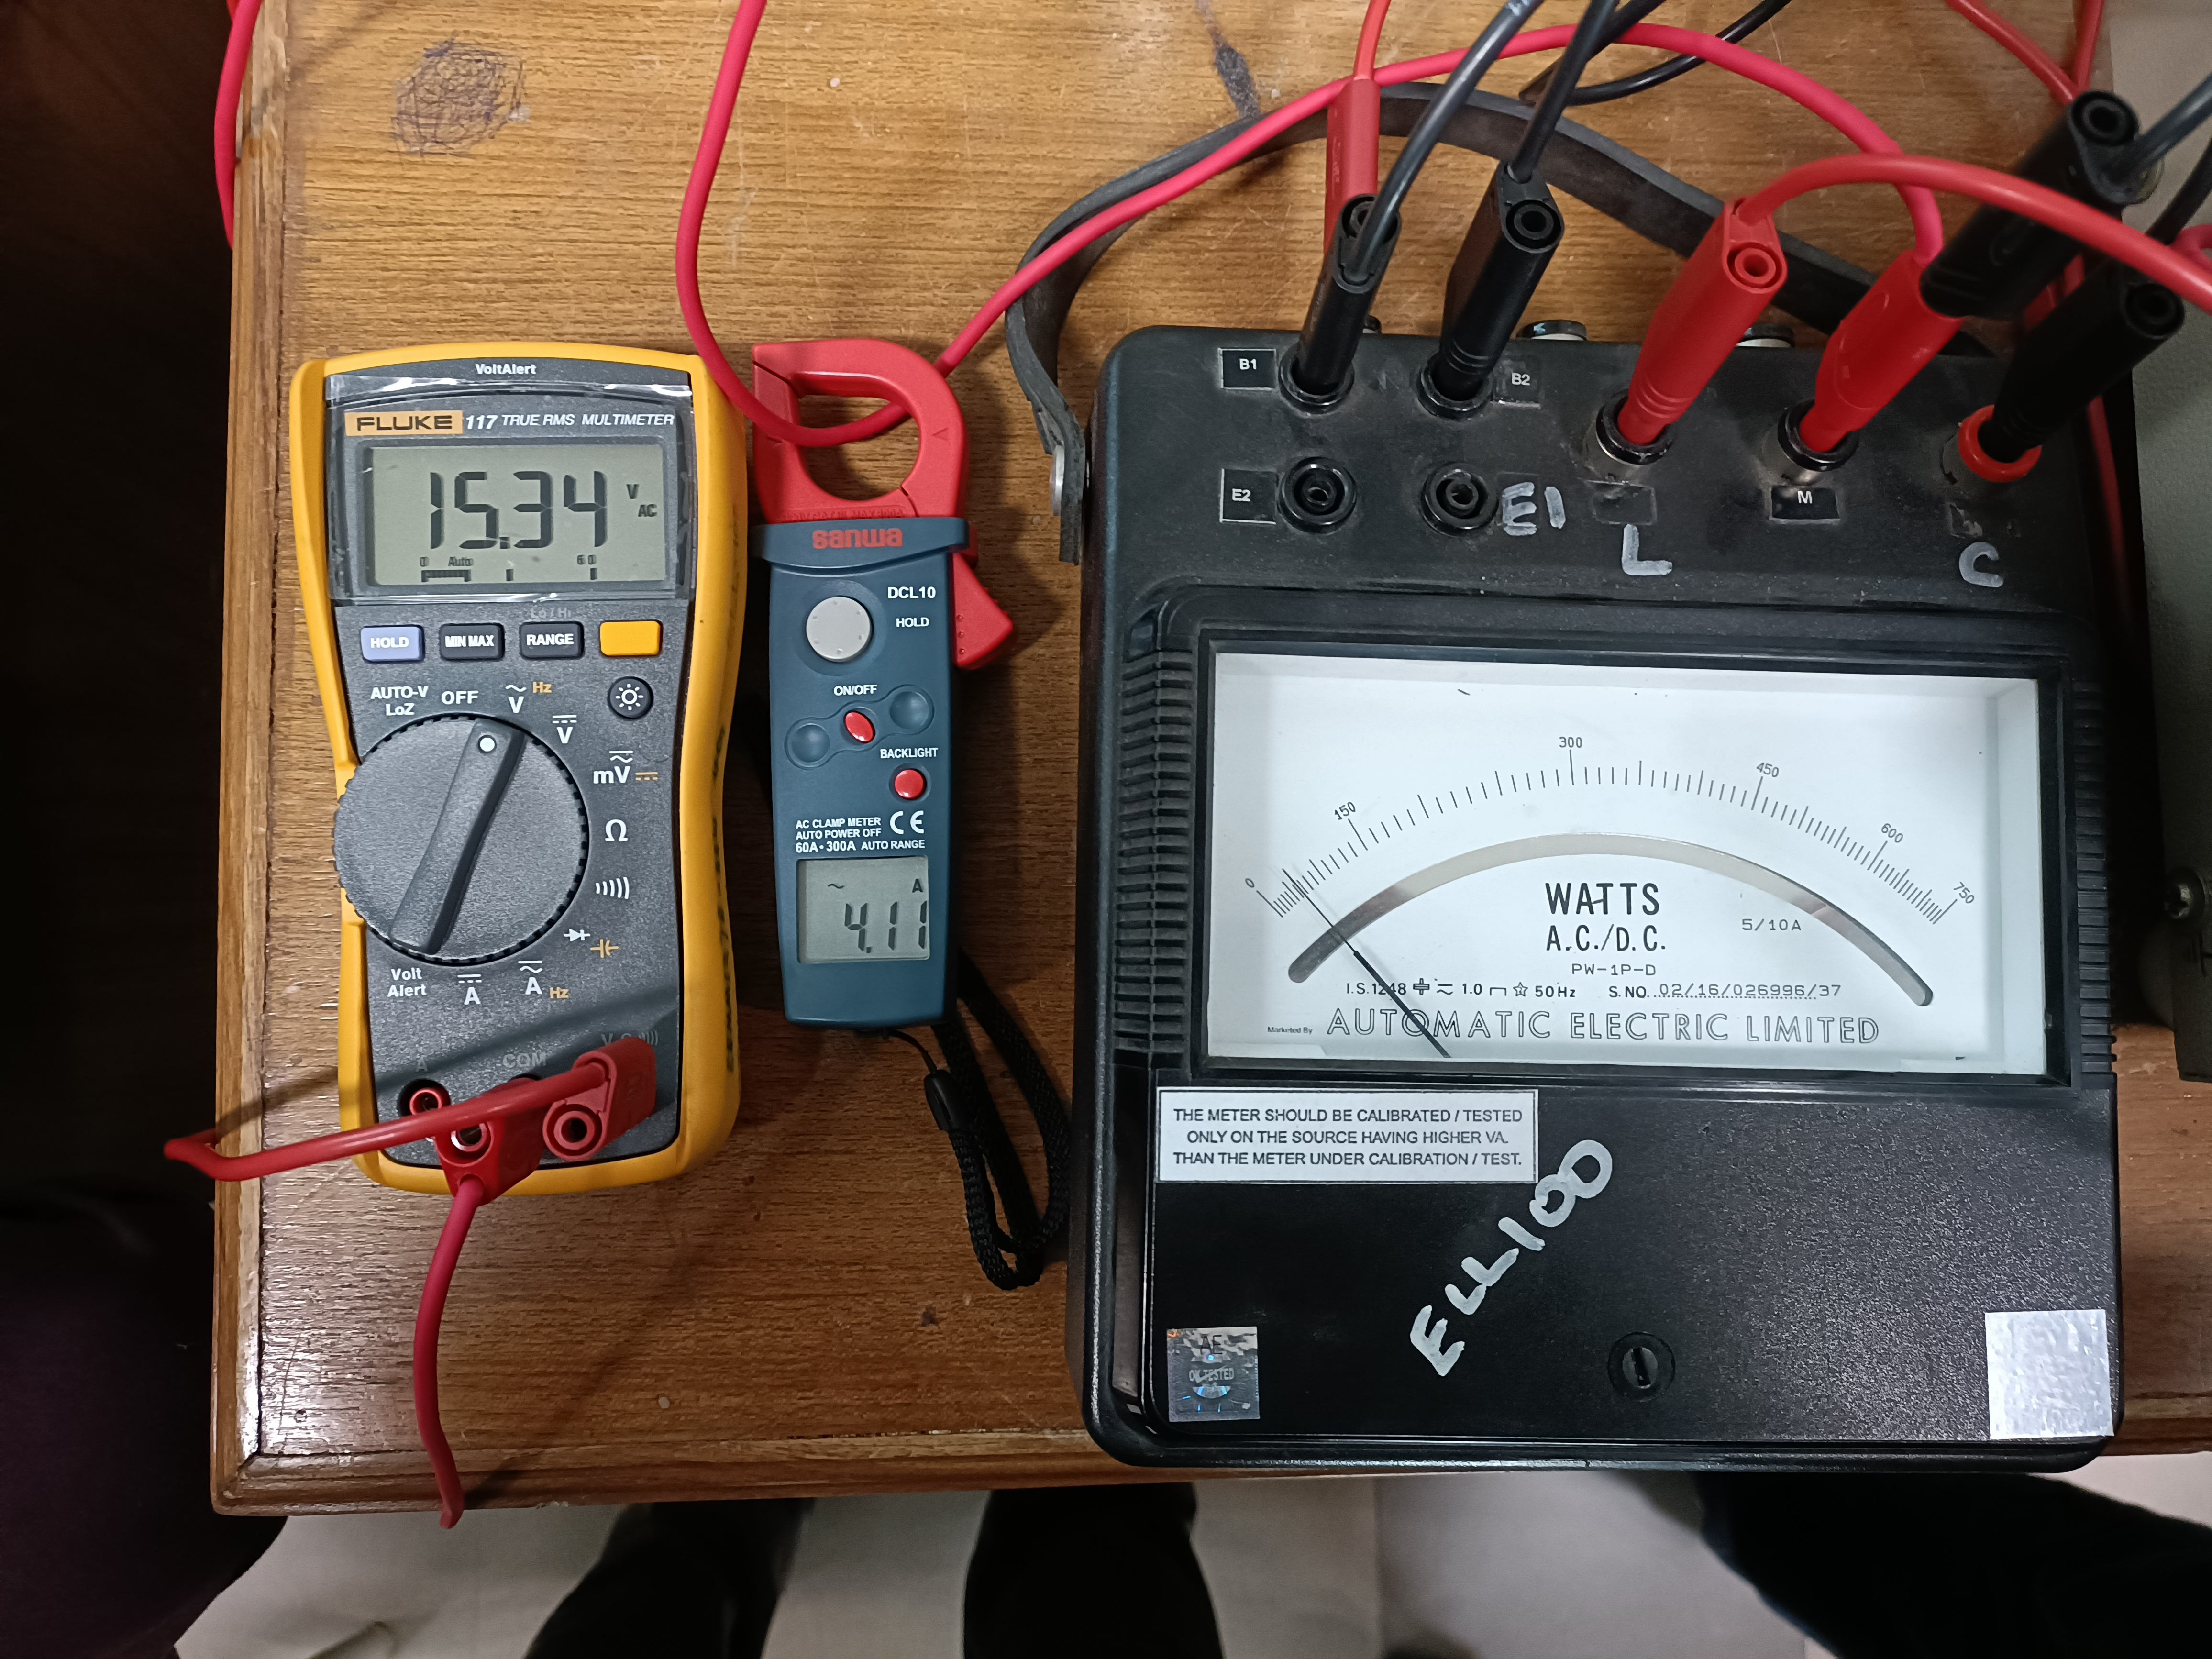
\includegraphics[width=0.35\textwidth]{IMG20220524160136.jpg}} & 15.28V & 4.12A & 60W \\
    \ & \ & \ & \ \\
 \hline
\end{tabular}
\end{center}
\newpage
\subsection{Calculation}
\begin{center}
OPEN CIRCUIT TEST \\
\vspace{10px}
\begin{tabular}{| c | c | c | c | c | c| c| c|} 
 \hline
    \ & \ & \ & \ & \ & \ & \ & \ \\
    $V_{Input}$ & $Current$ & $Power$ & $V_{Output}$ & $i_W$ & $i_\mu$ & $R_0$ & $X_0$\\ [1em]
    \hline
    \ & \ & \ & \ & \ & \ & \ & \ \\
    40.5V & 0.13A & 5.2W & 78.8V & 0.13A & 0.02A & 315.9 & 1934.1\\
    60.4V & 0.17A & 9.2W & 118.5V & 0.15A & 0.07A & 396.5 & 800.1\\
    81.3V & 0.21A & 14.6W & 159.7V & 0.18A & 0.10A & 452.7 & 746.8\\
    122.0V & 0.4A & 29.5W & 239.5V & 0.24A & 0.31A & 504.5 & 382.8\\
    \ & \ & \ & \ & \ & \ & \ & \ \\
 \hline
\end{tabular}
\end{center}
\vspace{10px}
\begin{center}
SHORT CIRCUIT TEST \\

\vspace{10px}
\begin{tabular}{| c | c | c | c | c | c|} 
 \hline
    \ & \ & \ & \ & \ & \ \\
    $V_{SC}$ & $I_{SC}$ & $Power$ & $Z_2$ & $R_2$ & $X_2$ \\ [1em]
    \hline
    \ & \ & \ & \ & \ & \ \\
    2.68V & 0.69A & 0W & 3.88 & 0 & 3.88 \\
    7.15V & 1.88A & 10W & 3.80 & 2.82 & 2.54\\
    10.9V & 2.89A & 30W & 3.77 & 3.59 & 1.15\\
    15.28V & 4.12A & 60W & 3.70 & 3.53 & 1.12\\
    \ & \ & \ & \ & \ & \ \\
 \hline
\end{tabular}
\end{center}
\vspace{10px}
\section{Sources of Error}
\begin{itemize}
\item Scale of DSO not appropriate for measurements
\item Loose Connections
\item Resistance of wires not taken into account, and also giving rise to inconsistency due to increase in resistance due to heating
\item Change in the connections while circuit is closed.

\end{itemize}

\vspace{5px}

\section{Precautions}

\begin{itemize}
\item Make the connections neat and tight
\item Don’t leave the switch on for long continuous periods of time.
\item Wear proper shoes and use insulated tools
\end{itemize}

\vspace{5px}

\section{Concluding Remarks}
From the above experiment, we have been able to calculate the various circuit parameters of a real transformer using the open circuit and the short circuit tests.

\vspace{10px}
\begin{center}
\fcolorbox{black}{white}{\includegraphics[width=0.8\columnwidth, height=200px]{Picture2.png}} \\ \vspace{5px}
\end{center}

For the given transformer, we calculated the absolute parameters as follows \\
$R_0$ = 5947.83 \\
$W_0$ = 1212.78 \\
$R_1$ = 1.11 \\
$R_2$ = 1.11 \\
$X_1$ = 1.95 \\
$X_2$ = 1.95 \\

\end{document}
